\part{监督学习}
监督学习是从标记的训练数据来推断一个功能的机器学习任务。训练数据包括一套训练示例。在监督学习中,每个实例都是由一个输入对象(通常为矢量)和一个期望的输出值(也称为监督信号)组成。监督学习算法是分析该训练数据,并产生一个推断的功能,其可以用于映射出新的实例。一个最佳的方案将允许该算法来正确地决定那些看不见的实例的类标签。这就要求学习算法是在一种“合理”的方式从一种从训练数据到看不见的情况下形成。

当采用了监督学习后,进一步确定目标变量若为离散值(标称量),则采用分类算法进行学习;若为连续值,则采用回归算法进行学习。

\section{分类}
监督学习的分类算法有很多,最简单的k-邻近算法,还有决策树,朴素贝叶斯,逻辑回归,支持向量机,Adaboost算法等。这些算法都有其特性,或多或少的公式推理,我都要去熟悉,学习,加实战。



\subsection{逻辑回归}

逻辑回归(Logistics Regression)是一种通过画出训练样本的决策边界,解决某种数据拟合二分类问题的有效途径。
对于怎样画出决策边界则为此算法核心。
我从逻辑函数(Logistic Function)的由来入手,学习了指数分布族,广义线性模型。

\subsubsection{指数分布簇}

介绍指数分布族(Exponential Family)为下一小节的广义线性模型(GLM)做铺垫。指数分布簇抽象统一形式为:
\begin{equation}
  p(y;\eta)=b(y)exp(\eta^T T(y)-a(\eta))
\end{equation}
其中参数$\eta$是自然常量;$T(y)$充分统计量(通常情况下$T(y)=y$);$a(\eta)$为对数划分函数;
给定三个函数$a(\eta),b(y),T(y)$就能确定一组概率分布;如在给定$\eta$值,便可以确定唯一一个概率分布。
那么有哪些常见分布属于指数分布族:
\begin{enumerate}
  \item 正态分布
  \item 二项分布
  \item 多项式分布
\end{enumerate}

\subsubsection{广义线性模型}
广义线性模型通过对指数分布族内分布进行建模得到响应函数从而得到目标函数,再通过某种最优化的算法(牛顿法/梯度上升法)得到最优系数,从而得到目标连接模型。
构建广义线性模型的步骤为,也就是广义线性模型的形式化定义为:
\begin{enumerate}
  \item $y|x;\theta \sim ExponentialFamily(\eta)$ \\即就是在给定$x,\theta$后,$y$满足的概率分布是以$\eta$为自然常数的指数分布族的一员。
  \item 给定x,输出~$h(x)=E[T(y)|x]$~即目标得到y的期望值。
  \item 最后令~$\eta=\theta^Tx$~(线性模型) 得到目标连接函数。
\end{enumerate}

现在以Bernoulli分布为例,构建广义线性模型,得到逻辑函数(也叫Sigmoid函数)。
现知道二项分布的概率密度函数为:
\begin{equation}\nonumber
\begin{split}
  p(y;\phi)&= \phi^y(1-\phi)^{1-y}\\
           &= exp~(yln\phi+(1-y)ln(1-\phi))\\
           &= exp~((ln(\frac{\phi}{1-\phi}))y+ln(1-\phi))
\end{split}
\end{equation}
对照指数分布族的抽象式(1)得到(这里~$\eta$~是标量):
\begin{equation}\nonumber
\begin{split}
  \eta   &=ln(\frac{\phi}{1-\phi}) \\
  T(y)   &= y\\
  a(\eta)&= -ln(1-\phi)\\
         &= ~ln(1+e^\eta)\\
  b(y)   &= 1\\
\end{split}
\end{equation}
得到关联函数:
\begin{equation}\nonumber
\begin{split}
  h_\theta(x) &= E(y|x;\theta)\\
              &= \phi~~~ (0-1~distribution's~mean)\\
              &= \frac{1}{1+e^{-\eta}}~~~(link function)\\
              &= \frac{1}{1+e^{-\theta^T x}}
\end{split}
\end{equation}

\subsubsection{理论:利用梯度上升做逻辑回归}
首先知道逻辑函数,所以令:
$$h_\theta(x)=g(\theta^T x)=\frac{1}{e^-\theta^Tx}$$
其中,
$$g(z)=\frac{1}{1+e^{-z}}$$
可以看出当~$z\rightarrow\infty~$时 ,$g(z)\rightarrow1$;当~$z\rightarrow-\infty~$时 ,$g(z)\rightarrow0$;
再令~$x_0=1$~,则:
$$\theta^Tx=\theta_0+\sum_{j=1}^{n}\theta_jx_j$$

$g(z)$~对z求导:
\begin{equation}
\begin{split}
  g'(z) &= \frac{\partial}{\partial z}\frac{1}{1+e^{-z}}\\
        &= \frac{1}{(1+e^{-z})^2}(e^{-z})\\
        &= \frac{1}{1+e^{-z}}\cdot(1-\frac{1}{(1+e^{-z})})\\
        &= g(z)(1-g(z))
\end{split}
\end{equation}

既然逻辑函数值表示概率,则:
\begin{equation}\nonumber
\begin{split}
  P(y=1|x;\theta) &= h_\theta(x)\\
  P(y=0|x;\theta) &= 1-h_\theta(x)
\end{split}
\end{equation}
即就是,
$$P(y|x;\theta)=(h_\theta(x))^y(1-h_\theta(x))^{1-y}$$
之后在对其进行极大似然估计:
\begin{equation}\nonumber
\begin{split}
  L(\theta) &= p(\overrightarrow{y}|X;\theta)\\
            &= \prod_{i=1}^{m}p(y^{(i)}|x^{(i)};\theta)\\
            &= \prod_{i=1}^{m}(h_\theta(x^{(i)}))^{y^{(i)}}(1-h_\theta(x^{(i)})^{1-y^{(i)}}\\
  l(\theta) &= ln L(\theta)\\
            &= \sum_{i=1}^{m}y^{(i)}lnh(x^{(i)})+(1-y^{(i)})ln(1-h(x^{(i)}))
\end{split}
\end{equation}
最终为了得到最大的~$l(\theta)$~,利用一种最优化算法梯度上升来求取,要求梯度,即求导:
\begin{equation}\nonumber
\begin{split}
  \frac{\partial}{\partial\theta_j}l(\theta) &= ( y\frac{1}{g(\theta^Tx)}-(1-y)\frac{1}{1-g(\theta^Tx)})\frac{\partial}{\partial\theta_j}g(\theta^Tx)\\
            &= ( y\frac{1}{g(\theta^Tx)}-(1-y)\frac{1}{1-g(\theta^Tx)})g(\theta^Tx)(1-g(\theta^Tx))\frac{\partial}{\partial\theta_j}\theta^Tx\\
            &= (y(1-g(\theta^Tx))-(1-y)g(\theta^Tx))x_j\\
            &= (y-h_\theta(x))x_j
\end{split}
\end{equation}
得到梯度后,再利用随机梯度上升(stochastic gradient ascent)迭代更新系数:
\begin{equation}\nonumber
\begin{split}
  \theta_j ~:=\theta_j+\alpha(y^{(i)}-h_\theta(x^{(i)}))x_j^{(i)}
\end{split}
\end{equation}

\subsubsection{实现:利用梯度上升做逻辑回归}
实战中利用的是梯度上升的最优化算法,逻辑回归就是利用最优化算法来训练出一个非线性函数用于分类。期间核心是利用最优化算法来寻找最佳拟合参数。
逻辑回归的优点是计算代价不高,易于理解与实现;其缺点是容易欠拟合,分类精度不高;适用数据类型是数值型与标称型数据。
逻辑回归的一般过程为:
\begin{enumerate}
  \item 收集数据:任意方法收集。
  \item 准备数据:最好为结构化数据。
  \item 分析数据:任意方法分析数据。
  \item 训练数据:大部分时间用来训练数据。
  \item 测试算法:测试会很快完成。
  \item 使用算法:输入数据,转结构化,进行回归计算,判定类别。
\end{enumerate}

\noindent\textbf{梯度上升找最佳参数~$\theta$~}\par
梯度上升算法的迭代公式如下,利用python实现。
\begin{equation}\nonumber
\begin{split}
  w := w +\alpha\nabla_wf(w)
\end{split}
\end{equation}

\noindent程序核心函数代码:
\begin{lstlisting}
def sigmoid(inX):
    return 1.0/(1+exp(-inX))

def gradAscent(dataMatIn, classLabels):
    dataMatrix = mat(dataMatIn)             #convert to NumPy matrix
    labelMat = mat(classLabels).transpose() #convert to NumPy matrix
    m,n = shape(dataMatrix)
    alpha = 0.001
    maxCycles = 600                         #Number of iterations
    weights = ones((n,1))
    for k in range(maxCycles):              #heavy on matrix operations
        h = sigmoid(dataMatrix*weights)     #matrix mult
        #print(dataMatrix*weights)          #$\eta$
        error = (labelMat - h)              #vector subtraction
        weights = weights + alpha * dataMatrix.transpose()* error #matrix mult
    return weights

def plotBestFit(weights):
    import matplotlib.pyplot as plt
    dataMat,labelMat=loadDataSet()
    dataArr = array(dataMat)
    n = shape(dataArr)[0]
    xcord1 = []; ycord1 = []
    xcord2 = []; ycord2 = []
    for i in range(n):
        if int(labelMat[i])== 1:
            xcord1.append(dataArr[i,1]); ycord1.append(dataArr[i,2])
        else:
            xcord2.append(dataArr[i,1]); ycord2.append(dataArr[i,2])
    fig = plt.figure()
    ax = fig.add_subplot(111)
    ax.scatter(xcord1, ycord1, s=30, c='red', marker='s')
    ax.scatter(xcord2, ycord2, s=30, c='green')
    x = arange(-3.0, 3.0, 0.1)
    y = (-weights[0]-weights[1]*x)/weights[2]
    ax.plot(x, y)
    plt.xlabel('X1'); plt.ylabel('X2');
    plt.show()
    plt.savefig('LogRegres_GradAscent.eps',dpi=2000)
\end{lstlisting}

利用测试数据得到初步的分类结果,并可视化表示结果如下图:
\begin{figure}[!hbt]
  \centering
  \includegraphics[width=0.6\textwidth]{1141.eps}
  \caption{利用梯度上升做逻辑回归的分类结果}
\end{figure}

\noindent分析图1:\\
\indent分类结果相当不错,从图中看上去只有四个点分类错误,但是知道一共需要600次迭代,也就是说至少要有600次的全训练数据的矩阵乘运算。
因此,不能将其作用于真实数据集的主要原因有二:其一时间复杂度缺陷;其二每一次迭代运算都需要作用于全体训练集,不利用扩充训练集。\\
接下来学习的随机梯度上升算法解决上述两类问题。

\noindent\textbf{随机梯度上升找最佳参数~$\theta$~}\par
随机梯度上升算法(Stochastic Gradient Ascent Algorithm)是一个在线学习算法,由于其可以在新样本到来时对分类器进行增量式的更新。与在线学习算法相对应的是,一次处理所有的数据被称为是批处理。\\
而随机梯度上升的迭代公式为:
\begin{equation}\nonumber
\begin{split}
  \theta_j ~:&=\theta_j+\alpha(y^{(i)}-h_\theta(x^{(i)}))x_j^{(i)}~~~~~~one~coefficient\\
  \Longrightarrow
  w :&= w+\alpha(y^{(i)}-h_\theta(x^{(i)}))x^{(i)}~~~~~~all~coefficient
\end{split}
\end{equation}

\noindent程序核心函数代码:
\begin{lstlisting}
def stocGradAscent0(dataMatrix, classLabels):
    m,n = shape(dataMatrix)
    # print (m,n)
    alpha = 0.01
    weights = ones(n)   #initialize to all ones
    for i in range(m):
        h = sigmoid(sum(dataMatrix[i]*weights))
        error = classLabels[i] - h
        weights = weights + alpha * error * dataMatrix[i] #Non matrix operation
    return weights
\end{lstlisting}

还是利用之前的测试数据得到初步的分类结果,并可视化表示结果如下图:
\begin{figure}[!hbt]
  \centering
  \includegraphics[width=0.6\textwidth]{1142.eps}
  \caption{利用随机梯度上升做逻辑回归的分类结果,并非最佳分类线}
\end{figure}

首先看回归系数与迭代次数的关系图:
\begin{figure}[!hbt]
  \centering
  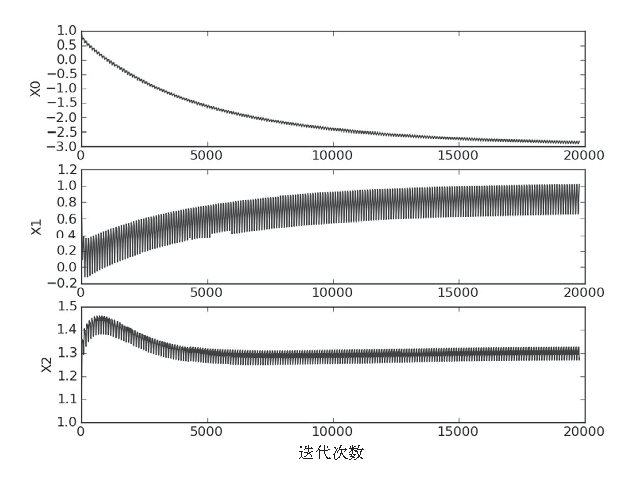
\includegraphics[width=0.65\textwidth]{1143.eps}
  \caption{回归系数与迭代次数的关系图}
\end{figure}

\noindent分析:\\
\indent分类器分错了三分之一的样本,但是只进行了类似于上节批量梯度下降的一次矩阵运算,所以结果并不公平。\\
\indent此外看到,存在一些不能正确分类的样本点,导致了在每次迭代的时,会引发系数的剧烈变化。
于是期望算法能避免来回波动,从而收敛到某个值;以及收敛的速度也应加快。
只要对其进行改进,效果则立竿见影。\\


\noindent\textbf{改进的随机梯度上升找最佳参数~$\theta$~}\par
\noindent程序核心函数代码:
\begin{lstlisting}
def stocGradAscent1(dataMatrix, classLabels, numIter=150):
    m,n = shape(dataMatrix)
    weights = ones(n)   #initialize to all ones
    for j in range(numIter):
        dataIndex = list(range(m))
        for i in range(m):
            alpha = 4/(1.0+j+i)+0.0001    #alpha decreases with iteration, does not
            randIndex = int(random.uniform(0,len(dataIndex)))#go to 0 because of the constant
            h = sigmoid(sum(dataMatrix[randIndex]*weights))
            error = classLabels[randIndex] - h
            weights = weights + alpha * error * dataMatrix[randIndex]
            del(dataIndex[randIndex])
            # print(dataIndex)
    return weights
\end{lstlisting}


还是利用之前的测试数据得到初步的分类结果,并可视化表示结果如下图:
\begin{figure}[!htb]
  \centering
  \includegraphics[width=0.6\textwidth]{1144.eps}
  \caption{利用改进的随机梯度上升做逻辑回归的分类结果}
\end{figure}


\noindent 算法参数分析:\\
\indent1.设置动态步长~$\alpha$~,缓解上节中数据的波动或者高频波动,比固定的$~\alpha~$收敛速度更快。当$~j<<max(i)~$时,$\alpha~$就不是严格下降,
避免参数的严格下降也常见于模拟退火算法等其他优化算法当中。\\
\indent2.训练样本随机选取更新回归系数,为了减少上节的周期性波动。

\begin{figure}[!htb]
  \centering
  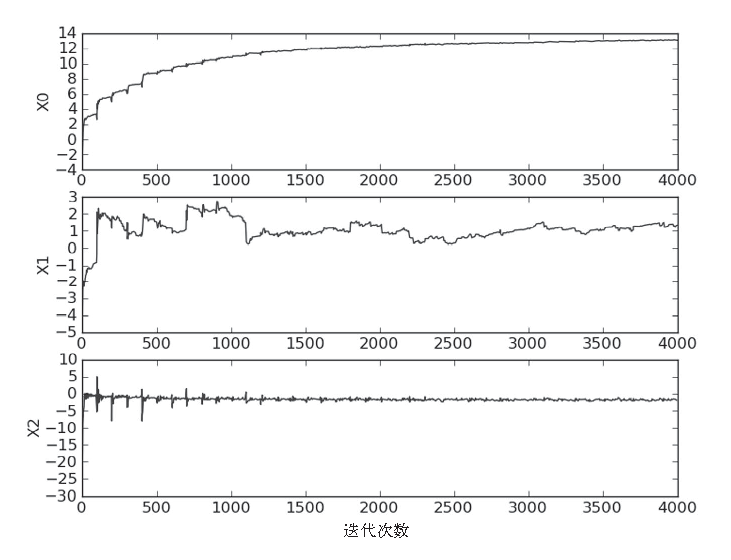
\includegraphics[width=0.65\textwidth]{1145.eps}
  \caption{改进算法后回归系数与迭代次数关系图}
\end{figure}

\noindent分析:\\
\indent改进的随机梯度下降优化算法与批量梯度下降优化算法相比,分类结果的效果差不多,但是所使用的计算量更少,
再利用小量的训练集时间差别不大,但是如果处理数以十亿计的训练样本和成千上万的特征时,两者的优越性则显露无疑。

\subsubsection{实战:利用逻辑回归,从疝气病症预测病马的死亡率}
将使用Logistic回归来预测患有疝病的马的存活问题。
这里数据包含368个样本,与28个特征;但有的指标比较主观,有的指标难以测量,例如马的疼痛级别。

另外,该数据有30\%的数据缺失用0填充,一条样本只有21个feature和1个label。\\
实战的步骤:
\begin{enumerate}
  \item 收集数据:给定数据文件。
  \item 准备数据:用python解析文本文件并填充缺失值。
  \item 分析数据:可视化并观察数据。
  \item 训练算法:使用优化算法,找到最佳的系数。
  \item 测试算法:观测错误率,回退调参,得到更好的回归系数。
  \item 使用算法:预测病马死亡率。
\end{enumerate}

\noindent\textbf{准备数据}\par
数据无价,数据中的缺失值,不能轻易的丢弃掉,有时也不能轻易的重新获取,必须采用一些方法来处理数据中的缺失值。这里采用的是使用特殊值来填充,用0填充,其对结果的预测不具有任何倾向性,因为$sigmoid(0)=0.5$。
\begin{enumerate}
  \item 使用特征均值填补缺失值。
  \item 使用特殊值来填补缺失值,如-1。
  \item 忽略有缺失值的样本。
  \item 使用相似样本的均值填补缺失值。
  \item 使用另外的机器学习算法预测缺失值。
\end{enumerate}

\noindent\textbf{测试算法}\par
将训练集中的数据进行逻辑回归分析,得出回归系数向量。在与特征向量相乘输入到sigmoid函数当中,结果大于0.5,预测为1;否则为0。\\
\noindent程序核心函数代码:
\begin{lstlisting}
def sigmoid(inX):
    if inX<-700:
        inX = -700    #avoid exp_function overflow
    return 1.0/(1+exp(-inX))

def stocGradAscent1(dataMatrix, classLabels, numIter=150):
    m,n = shape(dataMatrix)
    weights = ones(n)   #initialize to all ones
    for j in range(numIter):
        dataIndex = list(range(m))
        for i in range(m):
            alpha = 4/(1.0+j+i)+0.0001    #apha decreases with iteration, does not
            randIndex = int(random.uniform(0,len(dataIndex)))#go to 0 because of the constant
            h = sigmoid(sum(dataMatrix[randIndex]*weights))
            error = classLabels[randIndex] - h
            weights = weights + alpha * error * dataMatrix[randIndex]
            del(dataIndex[randIndex])
    # print("weight=",weights)
    return weights

def classifyVector(inX, weights):
    prob = sigmoid(sum(inX*weights))
    if prob > 0.5: return 1.0
    else: return 0.0

def colicTest():
    frTrain = open('horseColicTraining.txt'); frTest = open('horseColicTest.txt')
    trainingSet = []; trainingLabels = []
    for line in frTrain.readlines():
        currLine = line.strip().split('\t')
        lineArr =[]
        for i in range(21):
            lineArr.append(float(currLine[i]))
        trainingSet.append(lineArr)
        trainingLabels.append(float(currLine[21]))
    trainWeights = stocGradAscent1(array(trainingSet), trainingLabels, 1000)
    errorCount = 0; numTestVec = 0.0
    for line in frTest.readlines():
        numTestVec += 1.0
        currLine = line.strip().split('\t')
        lineArr =[]
        for i in range(21):
            lineArr.append(float(currLine[i]))
        if int(classifyVector(array(lineArr), trainWeights))!= int(currLine[21]):
            errorCount += 1
    errorRate = (float(errorCount)/numTestVec)
    print ("the error rate of this test is: %f" % errorRate)
    return errorRate

def multiTest():
    numTests = 10; errorSum=0.0
    for k in range(numTests):
        errorSum += colicTest()
    print ("after %d iterations the average error rate is: %f" % (numTests, errorSum/float(numTests)))
\end{lstlisting}

\noindent\textbf{预测结果}\par
\begin{lstlisting}
the error rate of this test is: 0.343284
the error rate of this test is: 0.328358
the error rate of this test is: 0.283582
the error rate of this test is: 0.298507
the error rate of this test is: 0.417910
the error rate of this test is: 0.417910
the error rate of this test is: 0.298507
the error rate of this test is: 0.358209
the error rate of this test is: 0.313433
the error rate of this test is: 0.343284
after 10 iterations the average error rate is: 0.340299
\end{lstlisting}

利用改进的随机梯度下降算法迭代求得回归系数,最终在作用于测试集,得到预测的平均错误率为34\%。这个结果相对不错,因为有30\%的数据缺失。事实上错误率还可以通过调参往下降。

\subsubsection{小结}
逻辑回归这一章从逻辑函数由来入手,学习了指数分布族,广义线性模型。知道逻辑函数是由bernoulli分布广义线性建模的结果。还给了必要的理论证明。

逻辑回归目的是寻找一个非线性函数Sigmoid的最佳拟合参数,求解过程可以由最优化算法来完成。最常用的就是梯度上升算法,而梯度上升算法可以改进为随机梯度上升算法。

随机梯度上升算法的效果相当,但占用更少的计算机资源。此外,随机梯度上升是一个在线算法,它可以在新的数据到来时就可以完成更新,而不需要重新读取整个数据集来进行批处理运算。

机器学习的一个重要的问题就是如何处理缺失数据。这个问题没有标准答案,取决于实际应用中的需求。现有的解决方案都各自有优缺点。

\newpage


\subsection{k-近邻算法}
k-近邻法(K-NN)是一种基本分类与回归方法,那么我现只接受了分类问题。此算法是一个多分类的机器学习算法,但是它是一个在线学习的算法,每一次做判别都要用到所有的训练集,寻找最小距离的训练样本。作为一个分类的“模型”,k 值的选择、距离度量及分类决策规则是k近邻法的三个基本要素。
\subsubsection{k近邻模型}
关于k近邻模型,我理解它是传统机器学习算法最简单的学习模型之一。k近邻法中,当训练集、距离度量(如欧氏距离〉、k值及分类决策规则(如多数表决〕确定后,对于任何一个新的输入实例,那么所属的类唯一地确定.这相当于根据上述要素将特征空间划分为一些子空间,确定于空间里的每个点所属的类。

\subsubsection{距离度量}
特征空间中两个实例点的距离是两个实例点相似程度的反映。k近邻模型的特征空间一般是n维实数向量空间$~R^n~$,使用的距离是欧氏距离,但也可以是其他距离, 如更一般的$~L_p~$距离$~(L_p~distance)~$或~Minkowski~距离(Minkowski~distance)。
\begin{align}
    L_p\text{距离}&: \nonumber\\
    &L_p(x_i,x_j)=\Big(\sum_{l=1}^{n}|x_i^{(l)}-x_j^{(l)}|^p\Big)^{\frac{1}{p}} \nonumber \\
    p=1~~~&\text{曼哈顿距离}:\nonumber \\
    &L_1(x_i,x_j)=\Big(\sum_{l=1}^{n}|x_i^{(l)}-x_j^{(l)}|\Big) \nonumber \\
    p=2~~~&\text{欧氏距离}:\nonumber\\
    &L_2(x_i,x_j)=\Big(\sum_{l=1}^{n}|x_i^{(l)}-x_j^{(l)}|^2\Big)^{\frac{1}{2}} \nonumber \\
    p=\infty~&~:\nonumber\\
    &L_\infty(x_i,x_j)=\max\limits_l |x_i^{(l)}-x_j^{(l)}| \nonumber 
\end{align}
下图表示二维空间中p取不同值时,与原点的$~L_p~$距离为1$~(L_p=1)~$的点的图形,
\begin{figure}
  \centering
  
\includegraphics[width=0.4\textwidth]{distance.eps}
  \caption{距离度量}
\end{figure}
那么显然\textcolor{red}{不同的距离度量所确定的最近邻点是不同的}。

\subsubsection{k值的选择}
k~值的选择会对k近邻法的结果产生重大影响。

如果选择较小的~k~值,对相近的实例点非常敏感,容易产生过拟合;相反地如果选择较大的~k~值,不相近的点也会起预测作用,使预测发生错误。

在应用中~k~值一般取一个比较小的数值.通常采用交叉验证法来选取最优的~k~值。通常~k~值是不大于20的整数。
\subsubsection{分类决策规则}
k~近邻法中的分类决策规则往往是多数表决,即由输入实例的~k~个邻近的训 练实例中的多数类决定输入实例的类。\textcolor{red}{事实上多数表决规则等价于经验风险最小化}。

\subsubsection{kd树}
实现k近邻法时,主要考虑的问题是\textcolor{red}{如何对训练数掘进行快速~k~近邻搜索},这点在特征空间的维数大及训练数据容量大时尤其必要。

k近邻法最简单的实现方法是线性扫描,这时要计算输入实例与每一个训练实例的距离当训练集很大时, 计算非常娓时,这种方法是不可行的.为了提高~k~近邻搜索的效率, 可以考虑使用特殊的数据结构存储 训练数据,以减少计算距离的次数。kd树就是一种较好的实现。

关于kd树的实现不详细记录,但要知道 如果实例点是随机分布的, kd树搜索的平均计算复杂度是$~O(logn)~$的 ,这里N是训练实例数。kd树更适用于训练实例数远大于空间维数时的~k~近邻搜索,当空间维数接近训练实例数时,它的效率会迅速下降,几乎成线性。

虽然 kd树的方法对于低维度$~(D<20)~$近邻搜索非常快,当D增长到很大时,效率变低: 这就是所谓的 “维度灾难” 的一种体现。

\subsubsection{实战:实现k近邻}
\noindent程序核心函数代码:
\begin{lstlisting}
def createDataSet():
    group = np.array([[1.0,1.1],[1.0,1.0],[0,0],[0,0.1]])
    labels = ['A','A','B','B']
    return group, labels

def classify0(inX, dataSet, labels, k):
    dataSetSize = dataSet.shape[0]   #training sample
    diffMat = np.tile(inX, (dataSetSize,1)) - dataSet   #difference
    sqDiffMat = diffMat**2   #square
    sqDistances = sqDiffMat.sum(axis=1)   #axis=1 row; 0 column
    distances = sqDistances**0.5   #root
    sortedDistIndicies = distances.argsort()   #sort to get index
    classCount={}
    for i in range(k):
        voteIlabel = labels[sortedDistIndicies[i]]
        classCount[voteIlabel] = classCount.get(voteIlabel,0) + 1  # value default 0
    sortedClassCount = sorted(classCount.items(), key=operator.itemgetter(1), reverse=True) #iterator,Specified sort field,Descending order
    return sortedClassCount
\end{lstlisting}

\noindent结果
\begin{lstlisting}
k=3
[('A', 2), ('B', 1)]
\end{lstlisting}


\subsubsection{实战:改进约会网站}
\noindent程序核心函数代码:
\begin{lstlisting}
def classify0(inX, dataSet, labels, k):
    dataSetSize = dataSet.shape[0]   #training sample
    diffMat = np.tile(inX, (dataSetSize,1)) - dataSet   #difference
    sqDiffMat = diffMat**2   #square
    sqDistances = sqDiffMat.sum(axis=1)   #axis=1 row; 0 column
    distances = sqDistances**0.5   #root
    sortedDistIndicies = distances.argsort()   #sort to get index
    classCount={}
    for i in range(k):
        voteIlabel = labels[sortedDistIndicies[i]]
        classCount[voteIlabel] = classCount.get(voteIlabel,0) + 1  # value default 0
    sortedClassCount = sorted(classCount.items(), key=operator.itemgetter(1), reverse=True) #iterator,Specified sort field,Descending order
    return sortedClassCount[0][0]

def file2matrix(filename):
    fr = open(filename)
    numberOfLines = len(fr.readlines())         #get the number of lines in the file
    returnMat = np.zeros((numberOfLines,3))        #prepare matrix to return
    classLabelVector = []                       #prepare labels return
    fr = open(filename)
    index = 0
    for line in fr.readlines():
        line = line.strip()
        listFromLine = line.split('\t')
        returnMat[index,:] = listFromLine[0:3]
        classLabelVector.append(int(listFromLine[-1]))
        index += 1
    return returnMat,classLabelVector

def autoNorm(dataSet):
    minVals = dataSet.min(0)
    maxVals = dataSet.max(0)
    ranges = maxVals - minVals
    normDataSet = np.zeros(np.shape(dataSet))
    m = dataSet.shape[0]
    normDataSet = dataSet - np.tile(minVals, (m,1))
    normDataSet = normDataSet/np.tile(ranges, (m,1))   #element wise divide
    return normDataSet, ranges, minVals

def datingClassTest():
    hoRatio = 0.50      #hold out 10%
    datingDataMat,datingLabels = file2matrix('datingTestSet2.txt')       #load data setfrom file
    normMat, ranges, minVals = autoNorm(datingDataMat)
    m = normMat.shape[0]
    numTestVecs = int(m*hoRatio)
    errorCount = 0.0
    for i in range(numTestVecs):
        classifierResult = classify0(normMat[i,:],normMat[numTestVecs:m,:]\
        ,datingLabels[numTestVecs:m],3)
        #print ("the classifier came back with: %d, the real answer is: %d" % (classifierResult, datingLabels[i]))
        if (classifierResult != datingLabels[i]): errorCount += 1.0
    print ("the total error rate is: %f" % (errorCount/float(numTestVecs)))
    print (errorCount)


if __name__=="__main__":
        datingClassTest()
\end{lstlisting}

\noindent结果:
\begin{lstlisting}
k=3
the total error rate is: 0.066000
\end{lstlisting}

\subsubsection{实战:手写字体的识别}
\noindent程序核心函数代码:
\begin{lstlisting}
def classify0(inX, dataSet, labels, k):
    dataSetSize = dataSet.shape[0]   #training sample
    diffMat = np.tile(inX, (dataSetSize,1)) - dataSet   #difference
    sqDiffMat = diffMat**2   #square
    sqDistances = sqDiffMat.sum(axis=1)   #axis=1 row; 0 column
    distances = sqDistances**0.5   #root
    sortedDistIndicies = distances.argsort()   #sort to get index
    classCount={}
    for i in range(k):
        voteIlabel = labels[sortedDistIndicies[i]]
        classCount[voteIlabel] = classCount.get(voteIlabel,0) + 1  # value default 0
    sortedClassCount = sorted(classCount.items(), key=operator.itemgetter(1), reverse=True) #iterator,Specified sort field,Descending order
    return sortedClassCount[0][0]
    
def handwritingClassTest():
    hwLabels = []
    trainingFileList = listdir('trainingDigits')           #load the training set
    m = len(trainingFileList)
    trainingMat = np.zeros((m,1024))
    for i in range(m):
        fileNameStr = trainingFileList[i]
        fileStr = fileNameStr.split('.')[0]     #take off .txt
        classNumStr = int(fileStr.split('_')[0])
        hwLabels.append(classNumStr)
        trainingMat[i,:] = img2vector('trainingDigits/%s' % fileNameStr)
    testFileList = listdir('testDigits')        #iterate through the test set
    errorCount = 0.0
    mTest = len(testFileList)
    for i in range(mTest):
        fileNameStr = testFileList[i]
        fileStr = fileNameStr.split('.')[0]     #take off .txt
        classNumStr = int(fileStr.split('_')[0])
        vectorUnderTest = img2vector('testDigits/%s' % fileNameStr)
        classifierResult = classify0(vectorUnderTest, trainingMat, hwLabels, 3)
        print ("the classifier came back with: %d, the real answer is: %d" % (classifierResult, classNumStr))
        if (classifierResult != classNumStr): errorCount += 1.0
    print ("\nthe total number of errors is: %d" % errorCount)
    print ("\nthe total error rate is: %f" % (errorCount/float(mTest)))
\end{lstlisting}
\noindent结果:
\begin{lstlisting}
the total number of errors is: 10
the total error rate is: 0.010571
Time For Run CompleteSMOWithKernel:34.74240867341453s compared with SVM 9s
\end{lstlisting}

\newpage
\subsection{高斯判别算法}
\subsubsection{生成学习算法}
逻辑回归或者感知机算法是在给定~x~的情况下直接对$~p(y|x;\theta)~$进行建模。其都是试图做分类边界,来进行分类;
那换个思路就是对各个分类目分别建立模型,最终将新样本输入到各个分类目模型当中去试图分类。

\noindent\textbf{判别学习算法}\par
判别学习算法(discriminative learning algorithm):直接学习$~p(y|x)~$或者是从输入直接映射到输出的方法;逻辑回归与感知机算法就是这一类算法的代表。

\noindent\textbf{生成学习算法}\par
生成学习算法(generative learning algorithm):对$~p(x|y)~$(也包括$~p(y)~$)进行建模。\\
建模方式:\\
输出两类:~~~~$y\in\{0,1\}$\\
$p(x|y=0):$~~~对0类特征进行建模\\
$p(x|y=1):$~~~对1类特征进行建模\\
完成对$~p(x|y)~$,以及$~p(y)~$的建模后。利用~Bayes~公式求得再给定~x~情况下~y~的概率,如下:
\begin{equation}\nonumber
\begin{split}
  &p(y|x)=\frac{p(x|y)p(y)}{p(x)}\\
  p(x)=p(x|y&=1)p(y=1)+p(x|y=0)p(y=0)
\end{split}
\end{equation}
最后再对$~p(x,y)~$进行最大似然估计,得到最佳参数。\\
最终将新样本输入到各个模型中得到概率值,判定类目。\\
事实上。可以不用完全算出概率值,比较不同类目输出结果大小即可。
\begin{equation}\nonumber
\begin{split}
  arg~\mathop{max}_y~p(y|x)&=arg~\mathop{max}_y\frac{p(x|y)p(y)}{p(x)}\\
  &=arg~\mathop{max}_y~p(x|y)p(y)\\
\end{split}
\end{equation}
常见的生成模型有:高斯判别分析(特征值为连续),隐马尔可夫模型HMM,朴素贝叶斯模型(特征值为离散),高斯混合模型GMM,LDA等。

\subsubsection{多项正太分布}
n维多项分布也称多项高斯分布,均值向量$~\mu\in R^n~$,协方差矩阵$~\Sigma\in R^{n\times n}~$,记为$~N(\mu,\Sigma)~$,其概率密度表示为:$$p(x;\mu,\Sigma)=\frac{1}{(2\pi)^{n/2}|\Sigma|^{1/2}}exp\Big(-\frac{1}{2}(x-\mu)^T\Sigma^{-1}(x-\mu)\Big)$$
其中$~|\Sigma|~$表示矩阵的行列式(determinant).\\
均值为$~E[X]=\displaystyle \int_xxp(x,;\mu,\Sigma)dx=\mu~$.\\
对于多元随机变量Z,$$~Cov(Z)=E[(Z-E[Z])(Z-E[Z])^T]=E[ZZ^T]-(E[Z])(E[Z])^T.~$$\\
则,$$If:~X\sim N(\mu,\Sigma)~$$$$So:~Cov(X)=\Sigma~$$

\noindent\textbf{二维正太分布图:} $\mu=[0,0],\Sigma=I$(单位阵)
\begin{figure}[!h]
  \centering
  \includegraphics[width=1\textwidth]{Gaussion1.eps}
  \caption{$\Sigma=I~~~~~~~~~~~~~~~~~~~~\Sigma=0.6I~~~~~~~~~~~~~~~~~~~~\Sigma=2I$}
\end{figure}

$$I=\begin{bmatrix}
      ~~1~ & ~0~~ \\
      ~~0~ & ~1~~
    \end{bmatrix}~~~~~~0.6I=\begin{bmatrix}
                      0.6 & 0 \\
                      0 & 0.6
                    \end{bmatrix}~~~~~~2I=\begin{bmatrix}
                                           ~~ 2~ & ~0~~ \\
                                           ~~ 0~ & ~2~~
                                          \end{bmatrix}$$

\begin{figure}[!h]
  \centering
  \includegraphics[width=1\textwidth]{Gaussion2.eps}
  \caption{$\Sigma=I~~~~~~~~~~~~~~~~~~~~\Sigma=I_1~~~~~~~~~~~~~~~~~~~~\Sigma=I_2$}
\end{figure}
$$I=\begin{bmatrix}
      ~~1~ & ~0~~ \\
      ~~0~ & ~1~~
    \end{bmatrix}~~~~~~I_1=\begin{bmatrix}
                      1 & 0.5 \\
                      0.5 & 1
                    \end{bmatrix}~~~~~~I_2=\begin{bmatrix}
                                            1 & 0.8 \\
                                            0.8 & ~1
                                          \end{bmatrix}$$

\newpage
\noindent\textbf{上图的等高线形式更能清晰可见:}
\begin{figure}[!h]
  \centering
  \includegraphics[width=1\textwidth]{GaussionO1.eps}
  \caption{$\Sigma=I~~~~~~~~~~~~~~~~~~~~\Sigma=I_1~~~~~~~~~~~~~~~~~~~~\Sigma=I_2$}
\end{figure}

\begin{figure}[!h]
  \centering
  \includegraphics[width=1\textwidth]{GaussionO2.eps}
  \caption{$\Sigma=I_3~~~~~~~~~~~~~~~~~~~~\Sigma=I_4~~~~~~~~~~~~~~~~~~~~\Sigma=I_5$}
\end{figure}
$$I_3=\begin{bmatrix}
      1 & -0.5 \\
      -0.5~ & 1
    \end{bmatrix}~~~~~~I_4=\begin{bmatrix}
                      1 & -0.8 \\
                      -0.8 & 1
                    \end{bmatrix}~~~~~~I_5=\begin{bmatrix}
                                            3 & 0.8 \\
                                            0.8 & 1
                                          \end{bmatrix}$$


\noindent\textbf{变均值,而不变协方差:}$\Sigma=I$
\begin{figure}[!h]
  \centering
  \includegraphics[width=1\textwidth]{Gaussion3.eps}
  \caption{$\mu=\mu_1~~~~~~~~~~~~~~~~~~~~\mu=\mu_2~~~~~~~~~~~~~~~~~~~~\mu=\mu_3$}
\end{figure}
$$\mu_1=\begin{bmatrix}
      1  \\
      0
    \end{bmatrix}~~~~~~\mu_2=\begin{bmatrix}
                      -0.5\\
                       0
                    \end{bmatrix}~~~~~~\mu_3=\begin{bmatrix}
                                            -1\\
                                            -0.5
                                          \end{bmatrix}$$

\noindent\textbf{因此,$~\mu~$决定中心位置,而$~\Sigma~$决定投影椭圆的朝向和大小。}

\subsubsection{高斯判别分析模型}
现有一个分类问题,训练集的特征值X都是随机的连续值,便可利用高斯判别模型(The Gaussian Discriminant Analysis model),假设:
\begin{equation}\nonumber
\begin{split}
  y &\sim Bernoulli(\phi)\\
  x|y=0 &\sim N(\mu_0,\Sigma)\\
  x|y=1 &\sim N(\mu_1,\Sigma)\\
\end{split}
\end{equation}
因此就有:
\begin{equation}\nonumber
\begin{split}
  p(y)&=\phi^y(1-\phi)^{1-y}\\
  p(x|y=0)&=\frac{1}{(2\pi)^{n/2}|\Sigma|^{1/2}}exp\bigg(-\frac{1}{2}(x-\mu_0)^T\Sigma^{-1}(x-\mu_0)\bigg)\\
  p(x|y=1)&=\frac{1}{(2\pi)^{n/2}|\Sigma|^{1/2}}exp\bigg(-\frac{1}{2}(x-\mu_1)^T\Sigma^{-1}(x-\mu_1)\bigg)\\
\end{split}
\end{equation}


\noindent最大似然估计$~l(\phi,\mu_0,\mu_1,\Sigma)~$得到最佳参数值:
\begin{equation}\nonumber
\begin{split}
  l(\phi,\mu_0,\mu_1,\Sigma)&=log\prod_{i=1}^{m}p(x^{(i)},y^{(i)};\phi,\mu_0,\mu_1,\Sigma)\\
  &=log\prod_{i=1}^{m}p(x^{(i)}|y^{(i)};\mu_0,\mu_1,\Sigma)p(y^{(i)};\phi)\\
\end{split}
\end{equation}
\begin{equation}\nonumber
\begin{split}
  \phi~&=\frac{1}{m}\sum_{i=1}^{m}{y^{i}=1}\\
  \mu_0&=\frac{\sum_{i=1}^{m}\textbf{1}\{y^{(i)}=0\}x^{(i)}}{\sum_{i=1}^{m}\textbf{1}\{y^{(i)}=0\}}\\
  \mu_1&=\frac{\sum_{i=1}^{m}\textbf{1}\{y^{(i)}=1\}x^{(i)}}{\sum_{i=1}^{m}\textbf{1}\{y^{(i)}=1\}}\\
  \Sigma&=\frac{1}{m}\sum_{i=1}^{m}(x^{(i)}-\mu_{y^{(i)}})(x^{(i)}-\mu_{y^{(i)}})^T\\
\end{split}
\end{equation}

\noindent理解公式(似然估计的结果非常简洁下节给出推导过程):\\
$~\phi~$:~训练集中分类结果为1所占的比例。\\
$~\mu_0~$:~$y=0$类样本中的特征均值。\\
$~\mu_1~$:~$y=1$类样本中的特征均值。\\
$\Sigma$:~是样本特征方差均值。\\

\noindent通过 上述的理论及描述,可以得到下面图像:\\
\begin{figure}[!htbp]
  \centering
  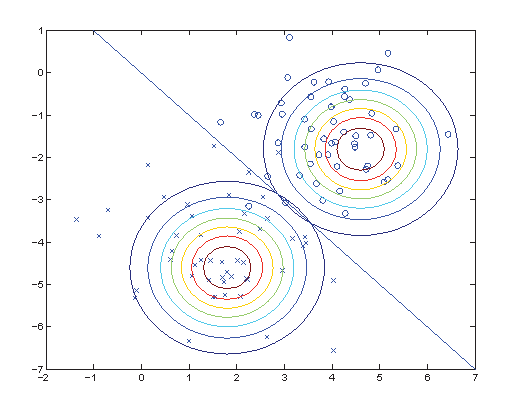
\includegraphics[width=0.6\textwidth]{GaussionOO.eps}
  \caption{高斯判别算法分类结果}
\end{figure}

\noindent分析:\\
直线两边的y值不同,但协方差矩阵相同,因此形状相同。$~\mu~$值不同,所以位置不同。

\subsubsection{GDA最大似然估计最佳参数详细推导}
\noindent对数似然函数:
\begin{equation}\nonumber
\begin{split}
  l(\phi,\mu_0,\mu_1,\Sigma)&=log\prod_{i=1}^{m}p(x^{(i)},y^{(i)})=log\prod_{i=1}^{m}p(x^{(i)}|y^{(i)})p(y^{(i)})=\sum_{i=1}^{m}log~p(x^{(i)}|y^{(i)})+log~p(y^{(i)})\\
                            &=\sum_{i=1}^{m}log~(p(x^{(i)}|y^{(i)}=0)^{1-y^{(i)}}\cdot p(x^{(i)}|y^{(i)}=1)^{y^{(i)}})+\sum_{i=1}^{m}log~p(y^{(i)})\\
                            &=\sum_{i=1}^{m}(1-y^{(i)})log~(p(x^{(i)}|y^{(i)}=0)+\sum_{i=1}^{m}y^{(i)}log~(p(x^{(i)}|y^{(i)}=1)+\sum_{i=1}^{m}log~p(y^{(i)})
\end{split}
\end{equation}
注意此函数分为三个部分,第一部分只与$~\mu_0~$有关;第二部分只与$~\mu_1~$有关;第三部分只$~\phi~$有关。最大化该函数,1.首先先求$~\phi~$,则求第三部分的偏导。
\begin{equation}\nonumber
\begin{split}
  \frac{\partial l(\phi,\mu_0,\mu_1,\Sigma)}{\partial\phi }&=\frac{\sum_{i=1}^{m}log~p(y^{(i)})}{\partial\phi}\\
   &=\frac{\partial\sum_{i=1}^{m}log~\phi^{y^{(i)}}(1-\phi)^{(1-y^{(i)})}}{\partial\phi}\\
   &=\frac{\partial\sum_{i=1}^{m}y^{(i)}log~\phi+(1-y^{(i)})log~(1-\phi)}{\partial\phi}\\
   &=\sum_{i=1}^{m}(y^{(i)}\frac{1}{\phi}-(1-y^{(i)})\frac{1}{1-\phi})\\
   &=\sum_{i=1}^{m}(I(y^{(1)}=1)\frac{1}{\phi}-I(y^{(i)}=0)\frac{1}{1-\phi})
\end{split}
\end{equation}
令其为零,求得$~\phi~$,(其中~I~是指示函数),
\begin{equation}\nonumber
\begin{split}
  {\color{red}{\phi=\frac{\sum_{i=1}^{m}I(y^{(i)}=1)}{m}}}
\end{split}
\end{equation}
2.同样地,对$~\mu_0~$求偏导,
\begin{equation}\nonumber
\begin{split}
  \frac{\partial l(\phi,\mu_0,\mu_1,\Sigma)}{\partial\mu_0}&=\frac{\partial\sum_{i=1}^{m}(1-y^{(i)})log~p(x^{(i)}|y^{(i)}=0)}{\partial\mu_0}\\
    &=\frac{\partial\sum_{i=1}^{m}(1-y^{(i)})(log\frac{1}{\sqrt{(2\pi)^2|\Sigma|}}-\frac{1}{2}(x^{(i)}-\mu_0)^T\Sigma^{-1}(x^{(i)}-\mu_0))}{\partial\mu_0}\\
    &=\sum_{i=1}^{m}(1-y^{(i)})\Sigma^{-1}(x^{(i)}-\mu_0)\\
    &=\sum_{i=1}^{m}I(y^{(i)}=0)\Sigma^{-1}(x^{(i)}-\mu_0)\\
\end{split}
\end{equation}
令其为0,得,
\begin{equation}\nonumber
\begin{split}
  {\textcolor{red}{\mu_0=\frac{\sum_{i=1}^{m}I\{y^{(i)}=0\}x^{(i)}}{\sum_{i=1}^{m}I\{y^{(i)}=0\}}}}\\
\end{split}
\end{equation}
3.同理得$~\mu_1~$,
\begin{equation}\nonumber
\begin{split}
  {\textcolor{red}{\mu_1=\frac{\sum_{i=1}^{m}I\{y^{(i)}=1\}x^{(i)}}{\sum_{i=1}^{m}I\{y^{(i)}=1\}}}}\\
\end{split}
\end{equation}
4.对$~\Sigma~$求偏导以求$~\Sigma~$(先改写初式前两部分),
\begin{equation}\nonumber
\begin{split}
  &\sum_{i=1}^{m}(1-y^{(i)})log~p(x^{(i)}|y^{(i)=0})+\sum_{i=1}^{m}y^{(i)}log~p(x^{(i)}|y^{(i)=1})\\
  =&\sum_{i=1}^{m}(1-y^{(i)})(log\frac{1}{\sqrt{(2\pi)^n|\Sigma|}}-\frac{1}{2}(x^{(i)}-\mu_0)^T\Sigma^{-1}(x^{(i)}-\mu_0))+\\
   &\sum_{i=1}^{m}y^{(i)}(log\frac{1}{\sqrt{(2\pi)^n|\Sigma|}}-\frac{1}{2}(x^{(i)}-\mu_1)^T\Sigma^{-1}(x^{(i)}-\mu_1))\\
  =& \sum_{i=1}^{m}log\frac{1}{\sqrt{(2\pi)^n|\Sigma|}}-\frac{1}{2}\sum_{i=1}^{m}(x^{(i)}-\mu_{y^{(i)}})^T\Sigma^{-1}(x^{(i)}-\mu_{y^{(i)}})\\
  =&\sum_{i=1}^{m}(-\frac{n}{2}log(2\pi)-\frac{1}{2}log(|\Sigma|))-\frac{1}{2}\sum_{i=1}^{m}(x^{(i)}-\mu_{y^{(i)}})^T(x^{(i)}-\mu_{y^{(i)}})
\end{split}
\end{equation}
进而有,
\begin{equation}\nonumber
\begin{split}
  \frac{\partial l(\phi,\mu_0,\mu_1,\Sigma)}{\partial\Sigma}&=-\frac{1}{2}\sum_{i=1}^{m}(\frac{1}{|\Sigma|}|\Sigma|\Sigma^{-1})-\frac{1}{2}\sum_{i=1}^{m}(x^{(i)}-\mu_{y^{(i)}})(x^{(i)}-\mu_{y^{(i)}})^T\frac{\partial\Sigma^{-1}}{\partial\Sigma}\\
  &=-\frac{m}{2}\Sigma^{-1}-\frac{1}{2}\sum_{i=1}^{m}(x^{(i)}-\mu_{y^{(i)}})(x^{(i)}-\mu_{y^{(i)}})^T(-\Sigma^{-2})\\
\end{split}
\end{equation}
这里用到的公式有,
\begin{equation}\nonumber
\begin{split}
  &\frac{\partial|\Sigma|}{\partial\Sigma}=|\Sigma|\Sigma^{-1}\\
  &\frac{\partial\Sigma^{-1}}{\partial\Sigma}=-\Sigma^{-2}\\
\end{split}
\end{equation}
令其为零,得,
\begin{equation}\nonumber
\begin{split}
  {\textcolor{red}{\Sigma=\frac{1}{m}\sum_{i=0}^{m}(x^{(i)}-\mu_{y^{(i)}})(x^{(i)}-\mu_{y^{(i)}})^T}}
\end{split}
\end{equation}

将参数全部求出后,可以看出公式推导相当复杂,但是结果是非常精简。
要判断一个新样本x时,可分别使用贝叶斯求出$~p(y=0|x)~$和$~p(y=1|x)~$,取概率更大的那个类。

实际计算时,我们只需要比大小,那么贝叶斯公式中分母项可以不计算,由于2个高斯函数协方差矩阵相同,则高斯分布前面那相同部分也可以忽略。实际上,GDA算法也是一个线性分类器,根据上面推导可以知道,GDA的分界线(面)的方程为:
\begin{equation}\nonumber
\begin{split}
  (1-\phi)exp((x-\mu_0)^T\Sigma^{-1}(x-\mu_0))=\phi exp((x-\mu_1)^T\Sigma(x-\mu_1))
\end{split}
\end{equation}
取对数展开后化解,可得:
\begin{equation}\nonumber
\begin{split}
  2x^T\Sigma^{-1}(\mu_1-\mu_0)=\mu_1^T\Sigma^{-1}\mu_1-\mu_0^T\Sigma^{-1}\mu_0+log\phi-log(1-\phi)
\end{split}
\end{equation}
若,
\begin{equation}\nonumber
\begin{split}
  A&=2\Sigma^{-1}(\mu_1-\mu_0)=(a_1,a_2,\ldots,a_n)\\
  B&=\mu_1^T\Sigma^{-1}\mu_1-\mu_0^T\Sigma^{-1}\mu_0+log\phi-log(1-\phi)\\
\end{split}
\end{equation}
则,
\begin{equation}\nonumber
\begin{split}
  a_1x_1+a_2x_2+\ldots+a_nx_n=b
\end{split}
\end{equation}
这就是GDA算法的线性分界面。
\subsubsection{高斯判别分析与逻辑回归对比}
\noindent似然公式对比:\\
GDA:
\begin{equation}\nonumber
\begin{split}
  l(\phi,\mu_0,\mu_1,\Sigma)&=log\prod_{i=1}^{m}p(x^{(i)},y^{(i)};\phi,\mu_0,\mu_1,\Sigma)\\
  &=log\prod_{i=1}^{m}p(x^{(i)}|y^{(i)};\mu_0,\mu_1,\Sigma)p(y^{(i)};\phi)\\
\end{split}
\end{equation}
LR:
\begin{equation}\nonumber
\begin{split}
  L(\theta) &= p(\overrightarrow{y}|X;\theta)\\
            &= \prod_{i=1}^{m}p(y^{(i)}|x^{(i)};\theta)\\
            &= \prod_{i=1}^{m}(h_\theta(x^{(i)}))^{y^{(i)}}(1-h_\theta(x^{(i)})^{1-y^{(i)}}\\
  l(\theta) &= ln L(\theta)\\
            &= \sum_{i=1}^{m}y^{(i)}lnh(x^{(i)})+(1-y^{(i)})ln(1-h(x^{(i)}))
\end{split}
\end{equation}

\noindent结论一:\\
如果$~x|y~\sim~Gaussian~$即其服从正太分布,那么它的后验公式$~p(y=1|x)~$就是逻辑函数(sigmoid function)。\\
证明:\\
由贝叶斯公式可知:
\begin{equation}\nonumber
\begin{split}
  p(y=1|x)&=\frac{p(x|y=1)p(y=1)}{p(x)}\\
          &=\frac{N(\mu_1,\Sigma)\phi}{N(\mu_0,\Sigma)(1-\phi)+N(\mu_1,\Sigma)\phi}\\
          &=1/(1+\frac{N(\mu_0,\Sigma)}{N(\mu_1,\Sigma)}\frac{1-\phi}{\phi})\\
\end{split}
\end{equation}
而:
\begin{equation}\nonumber
\begin{split}
  \frac{N(\mu_0,\Sigma)}{N(\mu_1,\Sigma)}&=exp\{(x-\mu_0)^T\Sigma^{-1}(x-\mu_0)-(x-\mu_1)^T\Sigma^{-1}(x-\mu)\}\\
  &=exp\{2(\mu_1-\mu_0)^T\Sigma^{-1}x+(\mu_0^T\Sigma \mu_0-\mu_1^T\Sigma\mu_1)\}
\end{split}
\end{equation}
那么,令:
\begin{equation}\nonumber
\begin{split}
  &2\Sigma^{-1}(\mu_1-\mu_0)=(\theta_1,\theta_2,......,\theta_n)^T\\
  &\theta_0=\mu_0^T\Sigma\mu_0-\mu_1^T\Sigma\mu_1+log\frac{1-\phi}{\phi}
\end{split}
\end{equation}
则:
\begin{equation}\nonumber
\begin{split}
  p(y=1|x)=\frac{1}{1+exp(\theta_0+\theta_1x_1+\theta_2x_2+...+\theta_nx_n)}
\end{split}
\end{equation}
结论一得证。

\noindent结论二:\\
\begin{equation}\nonumber
\left\{
\begin{aligned}
\overset{.}x|y=1\sim Possion(\lambda_1) \\
x|y=0\sim Possion(\lambda_0)\\
\end{aligned}
\right.
\end{equation}
$$\Rightarrow p(y=1|x)\rightarrow logistic function.$$

在推导逻辑回归的时候,我们并没有假设类内样本是服从高斯分布的,因而GDA只是逻辑回归的一个特例,其建立在更强的假设条件下。故两者效果比较:\\
1.逻辑回归是基于弱假设推导的,则其效果更稳定,适用范围更广。\\
2.数据服从高斯分布时,GDA效果更好。\\
3.当训练样本数很大时,根据中心极限定理,数据将无限逼近于高斯分布,则此时GDA的表现效果会非常好。\\

\noindent\textbf{为何要假设两类内部高斯分布的协方差矩阵相同?}\\
从直观上讲,假设两个类的高斯分布协方差矩阵不同,会更加合理(在混合高斯模型中就是如此假设的),而且可推导出类似上面简洁的结果。\\
假定两个类有相同协方差矩阵,分析具有以下几点影响:\\
1.当样本不充分时,使用不同协方差矩阵会导致算法稳定性不够;过少的样本甚至导致协方差矩阵不可逆,那么GDA算法就没法进行\\
2.使用不同协方差矩阵,最终GDA的分界面不是线性的,同样也推导不出GDA的逻辑回归形式\\

\noindent\textbf{使用GDA时对训练样本有何要求?}\\
1.正负样本数的比例需要符合其先验概率。若是预先明确知道两类的先验概率,那么可使用此概率来代替GDA计算的先验概率;若是完全不知道,则可以公平地认为先验概率为50\%.\\
2.样本数必须不小于样本特征维数,否则会导致协方差矩阵不可逆,按照前面分析应该是多多益善。

\newpage
\subsection{朴素贝叶斯算法}
朴素贝叶斯(naive Bayes)法是基于\textbf{贝叶斯定理}与\textbf{特征条件独立假设}的分类方法。对于给定的训练数据集,首先基于特征条件独立假设学习输入/输出的联合概率分布;然后基于此模型,对于给定的输入~x,利用贝叶斯定理求出后验概率最大的输出~y。当然,朴素贝叶斯算法与高斯判别法一样也是一种典型的生成学习算法。

\subsubsection{概率论基础}
贝叶斯学派的思想可以概括为先验概率+数据=后验概率。\\
\noindent\textbf{条件独立公式}\\
$$P(X,Y)=P(X)P(Y)$$
\noindent\textbf{条件概率公式}\\
$$P(Y|X)=P(X,Y)/P(X)$$
$$P(X|Y)=P(Y,X)/P(Y)$$
$$P(X|Y)=\frac{P(Y|X)P(X)}{P(Y)}$$
\noindent\textbf{全概率公式}\\
$$P(X)=\sum_{i=1}^{m}P(X|Y=Y_i)P(Y_i)~~,~~\sum_{i=1}^{m}Y_i=1$$
\noindent\textbf{贝叶斯公式}\\
$$P(Y_j|X)=\frac{P(X|Y_j)P(Y_j)}{\sum_{i=1}^{m}P(X|Y=Y_i)P(Y_i)}$$
其中,\\
$P(Y_j)~$为先验概率;\\
$P(X|Y_j)~$为似然函数;\\
$P(X)~$为归一化项;\\
$P(Y_j|X)~$为后验概率;\\

那么朴素贝叶斯算法的核心就是,利用最大似然估计,求取$~P(X|Y_j)~$,最终比较后验概率大小来判别类别。
\subsubsection{算法数学原理流程}
利用上述概率论基础,回到我们的数据分析,来构我们的建朴素贝叶斯分类器。\\
假设我们\textbf{有m个样本},每个样本有n个特征,特征输出有两个类别,定义为1,0.(多分类同理)。
$$(x_1^{(1)},x_2^{(1)},...,x_n^{(1)},y_1),(x_1^{(2)},x_2^{(2)},...,x_n^{(2)},y_2),...,(x_1^{(m)},x_2^{(m)},...,x_n^{(m)},y_m)$$
从这些样本中就可以学习到\textbf{朴素贝叶斯的先验分布}$~P(Y=1),P(Y=0)~$;接着可以学习\textbf{条件概率分布}$~P(X|Y=0),P(X|Y=1)~$;这里就出现了一个问题,多元变量n个维度的条件分布很难求出。所以朴素贝叶斯就用到了一个大胆的\textbf{强独立假设(Naive Bayes Assumption)},样本各个特征之间相互独立则有:
\begin{equation}\nonumber
\begin{split}
  P(X|Y_j)&=P(x_1,x_2,...,x_n|Y_j)\\
            &=P(x_1|Y_j)P(x_2|Y_j)...P(x_n|Y_j)\\
            &=\prod_{i=1}^{n}P(x_i|Y_j)
\end{split}
\end{equation}
从上式可以看出,这个很难的条件分布大大的简化了,但是这也可能带来预测的不准确性。你会说如果我的特征之间非常不独立怎么办?如果真是非常不独立的话,那就尽量不要使用朴素贝叶斯模型了,考虑使用其他的分类方法比较好。但是一般情况下,样本的特征之间独立这个条件的确是弱成立的,尤其是数据量非常大的时候。虽然我们牺牲了准确性,但是得到的好处是模型的条件分布的计算大大简化了,这就是贝叶斯模型的选择。\\
那么现在朴素贝叶斯可可将贝叶斯公式重写为:
\begin{equation}\nonumber
\begin{split}
  P(Y_j|X)&=\frac{P(X|Y_j)P(Y_j)}{\sum_{i=1}^{m}P(X|Y=Y_i)P(Y_i)}\\
          &=\frac{\prod_{i=1}^{n}P(x_i|Y_j)P(Y_j)}{\sum_{i=1}^{m}P(X|Y=Y_i)P(Y_i)}\\
          &=\frac{\prod_{i=1}^{n}P(x_i|Y_j)P(Y_j)}{...}
\end{split}
\end{equation}
将分母省略实际上,是在朴素贝叶斯算法判别时是比较大小时,各类的后验概率都不用去除以相同的归一化项,可直接用来比较。事实上,此模型还用到了一个假设就是\textbf{特征同等重要假设}。

\subsubsection{多元变量伯努利事件模型(词集模型)}%词集模型 (不考虑频次)
\noindent\textbf{1.词集模型:}\\
\indent多元变量伯努利事件模型(multi-variate Bernoulli event model)常用于文本分类,也称为\textbf{词集模型(set-of-words model)}就是不考虑同一文档中同一特征出现的频率,只要出现就将其置1。具体的建模过程为:\\
\textcircled{\footnotesize{1}}模型总词表:(长度为n=5000)
$$Vocabulary=[word_1,word_2,...,word_{5000}]$$
\textcircled{\footnotesize{2}}文档词向量:(长度为n=5000,与总词表对应,存在文档总词表的单词相应位置置1)
$$WordVector=[0,0,1,0,1,0,0,...1,0]$$
\textcircled{\footnotesize{3}}特征为离散二值变化,输出也是二值\{0,1\}。因此有:
\begin{equation}\nonumber
\begin{split}
  &\phi_y=p(y=1)\\
  &\phi_{j|y=0}=p(x_j=1|y=1)\\
  &\phi_{j|y=1}=p(x_j=0|y=0)\\
\end{split}
\end{equation}
\textcircled{\footnotesize{4}}将$~y~$和$~x_j,y~$建模成Bernoulli分布(这是朴素贝叶斯最简单的特例之一),
\begin{equation}\nonumber
\begin{split}
  &p(y)=(\phi_y)^y(1-\phi_y)^{1-y}\\
  &p(x|y=0)=\prod_{j=1}^{n}p(x_j|y=0)=\prod_{j=1}^{n}(\phi_{j|y=0})^{x_j}(1-\phi_{j|y=0})^{1-x_j}\\
  &p(x|y=1)=\prod_{j=1}^{n}p(x_j|y=1)=\prod_{j=1}^{n}(\phi_{j|y=1})^{x_j}(1-\phi_{j|y=1})^{1-x_j}\\
\end{split}
\end{equation}
\textcircled{\footnotesize{5}}强独立假设下的似然函数(有m个样本):
\begin{equation}\nonumber
\begin{split}
  L(\phi_y,\phi_{i|y=1},\phi_{i|y=0})&=\prod_{i=1}^{m}p(x^{(i)},y^{(i)};\phi_y,\phi_{i|y=1},\phi_{i|y=0})\\
\end{split}
\end{equation}
{\color{red}{\textcircled{\footnotesize{6}}}最大似然求参数:}
\begin{equation}\nonumber
\begin{split}
  l(\phi_y,\phi_{i|y=1},\phi_{i|y=0})&=log\prod_{i=1}^{m}p(x^{(i)},y^{(i)};\phi_y,\phi_{i|y=1},\phi_{i|y=0})\\
                                     &=log\prod_{i=1}^{m}p(y^{(i)};\phi_y)p(x^{(i)}|y^{(i)};\phi_{j|y=0},\phi_{j|y=1})\\
                                     &=\sum_{i=1}^{m}\Big(log(\phi_y^{y^{(i)}}(1-\phi_y)^{1-y^{(i)}})+log\prod_{j=1}^{n}p(x_j^{(i)}|y^{(i)})\Big)\\
                                     &=\sum_{i=1}^{m}\Big((y^{(i)}log\phi_y+(1-y^{(i)})log(1-\phi_y))\\
                                     &~~~~~+log\prod_{j=1}^{n}(p(x_j^{(i)}|y^{(i)}=1))^{I\{y^{(i)}=1\}}(p(x_j^{(i)}|y^{(i)}=0))^{I\{y^{(i)}=0\}}\Big)\\
                                     &=\sum_{i=1}^{m}\Big((y^{(i)}log\phi_y+(1-y^{(i)})log(1-\phi_y))\\
                                     &~~~~~+\sum_{j=1}^{n}I\{y^{(i)}=1\}log~p(x_j^{(i)}|y^{(i)}=1)\\
                                     &~~~~~~~~~~+\sum_{j=1}^{n}I\{y^{(i)}=0\}log~p(x_j^{(i)}|y^{(i)}=0)\Big)\\
                                     &=\sum_{i=1}^{m}\Big((y^{(i)}log\phi_y+(1-y^{(i)})log(1-\phi_y))\\
                                     &~~~~~+\sum_{j=1}^{n}I\{y^{(i)}=1\}log~(\phi_{j|y=1})^{x_j^{(i)}}(1-\phi_{j|y=1})^{1-x_j^{(i)}}\\
                                     &~~~~~~~~~~+\sum_{j=1}^{n}I\{y^{(i)}=0\}log~(\phi_{j|y=0})^{x_j^{(i)}}(1-\phi_{j|y=0})^{1-x_j^{(i)}}\Big)\\
\end{split}
\end{equation}
全式分为三部分,为求$~\phi_y~$对第一部分求导:
\begin{equation}\nonumber
\begin{split}
  &\frac{\partial l}{\partial \phi_y}=\sum_{i=1}^{m}\frac{y^{(i)}}{\phi_y}-\frac{1-y^{(i)}}{1-\phi_y} =0\\
  &{\color{red}{\Rightarrow\phi_y = \frac{\sum_{i=1}^{m}I\{y^{(i)}=1\}}{m}}}\\
\end{split}
\end{equation}
为求$\phi_{j|y=1}$对第二部分求导:
\begin{equation}\nonumber
\begin{split}
  \frac{\partial l}{\partial \phi_{j|y=1}}&= \frac{\partial \sum_{i=1}^{m}I\{y^{(i)}=1\}log~(\phi_{j|y=1})^{x_j^{(i)}}(1-\phi_{j|y=1})^{1-x_j^{(i)}}}{\partial \phi_{j|y=1}}\\
  &=\sum_{i=1}^{m}I\{y^{(i)}=1\}(\frac{x_j^{(i)}}{\phi_{j|y=1}}-\frac{1-x_j^{(i)}}{1-\phi_{j|y=1}})=0\\
  \Rightarrow~&{\color{red}{\phi_{j|y=1}=\frac{\sum_{i=1}^{m}I\{y^{(i)}=1\wedge x_j^{(i)}=1\}}  {\sum_{i=1}^{m}I\{y^{(i)}=1\}}}}\\
\end{split}
\end{equation}
同理,可得$\phi_{j|y=0}$:
\begin{equation}\nonumber
\begin{split}
  &{\color{red}{\phi_{j|y=0}=\frac{\sum_{i=1}^{m}I\{y^{(i)}=0\wedge x_j^{(i)}=1\}}  {\sum_{i=1}^{m}I\{y^{(i)}=0\}}}}\\
\end{split}
\end{equation}
所以,我们得到了模型所有的参数值(进行拉普拉斯平滑后的结果);可以利用贝叶斯公式判别新样本类别:
\begin{equation}\nonumber
\begin{split}
  &\phi_y = \frac{\sum_{i=1}^{m}I\{y^{(i)}=1\}{\color{red}{+1}}}{m{\color{red}{+2}}}\\
  &\phi_{j|y=1}=\frac{\sum_{i=1}^{m}I\{y^{(i)}=1\wedge x_j^{(i)}=1\}{\color{red}{+1}}}{\sum_{i=1}^{m}I\{y^{(i)}=1\}{\color{red}{+2}}}\\
  &\phi_{j|y=0}=\frac{\sum_{i=1}^{m}I\{y^{(i)}=0\wedge x_j^{(i)}=1\}{\color{red}{+1}}}{\sum_{i=1}^{m}I\{y^{(i)}=0\}{\color{red}{+2}}}\\
\end{split}
\end{equation}


\noindent最后,\textbf{上述建模的贝叶斯分类器,是一个线性分类器};\\即存在某个$\theta\in R^{(n+1)}$,(特征第0个位置,对应截距项$\theta_0$)
$$p(y=1|x)>=p(y=0|x)~\Leftrightarrow~\theta^T \begin{bmatrix}
   1  \\
   x
  \end{bmatrix}>=0$$
证明:
\begin{equation}\nonumber
\begin{split}
  &p(y=1|x)>=p(y=0|x)\\
  \Leftrightarrow&\frac{p(y=1|x)}{p(y=0|x)}>=1\\
  \Leftrightarrow&\frac{(\prod_{j=1}^{n}p(x_j|y=1))p(y=1)}{(\prod_{j=1}^{n}p(x_j|y=0))p(y=0)}>=1\\
  \Leftrightarrow&\frac{(\prod_{j=1}^{n}(\phi_{j|y=1})^{x_j}(1-\phi_{j|y=1})^{(1-x_j)})\phi_y}{(\prod_{j=1}^{n}(\phi_{j|y=0})^{x_j}(1-\phi_{j|y=0})^{(1-x_j)})(1-\phi_y)}>=1\\
  \Leftrightarrow&\sum_{j=0}^{n}x_j log(\phi_{j|y=1})+(1-x_j)log(1-\phi_{j|y=1})+log\phi_y\\
  ~~~~~~~~~~&-\sum_{j=0}^{n} x_j log(\phi_{j|y=0})+(1-x_j)log(1-\phi_{j|y=0})+(1-log\phi_y)>=0\\
  \Leftrightarrow&\sum_{j=1}^{n}x_jlog\frac{\phi_{j|y=1}}{(1-\phi_{j|y=1})}+log(1-\phi_{j|y=1})\\
  ~~~~~~~~~~&-\sum_{j=1}^{n}x_jlog\frac{\phi_{j|y=0}}{(1-\phi_{j|y=0})}-log(1-\phi_{j|y=0})+log\frac{\phi_y}{1-\phi_y}>=0\\
  \Leftrightarrow&\sum_{j=1}^{n}x_jlog\frac{\phi_{j|y=1}(1-\phi_{j|y=0})}{(1-\phi_{j|y=1})\phi_{j|y=0}}+log\frac{\phi_y}{1-\phi_y}>=0\\
\end{split}
\end{equation}
此时:$$\theta_0 = \sum_{j=1}^{m} log\frac{1-\phi_{j|y=1}}{1-\phi_{j|y=0}}+log\frac{\phi_y}{1-\phi_y}$$
$$\theta_j=\frac{\phi_{j|y=1}(1-\phi_{j|y=0})}{(1-\phi_{j|y=1})\phi_{j|y=0}}$$
也就是说,{\color{red}{我们拿一个新数据x代入模型测试,利用我们上面得到的线性分类器$\theta^Tx$,与利在朴素贝叶斯比较$p(y=1|x)$与$p(y=0|x)$是等效的。}}\textbf{事实上,离散特征的朴素贝叶斯分类器都是线性分类器;方差相同的连续的朴素贝叶斯分类器也是线性分类器。}进一步讲,只有某些具有特定属性的朴素贝叶斯分类器才是线性分类器。

\subsubsection{多项式事件模型(词袋模型)} %词袋模型(考虑到频次)-多用于文本分类问题
多项式事件模型(multinomial event model)又称为朴素贝叶斯的词袋模型(多用于文档分类),\textbf{词袋模型(bag-of-words model)}就是考虑同一文档中重复出现的词以累加,显然词袋模型更加贴合实际;其建模过程,与伯努利事件模型相像,只是特征不在只取二值,而是多值$\{1,2,3,4,...\}$。这就与伯努利事件模型出现了差异,\textbf{其每一个特征变量不在服从伯努利分布而是多项式分布。}最大似然的过程相似,但结果不同,其似然结果为:
\begin{equation}\nonumber
\begin{split}
  &\phi_y = \frac{\sum_{i=1}^{m}I\{y^{(i)}=1\}{\color{red}{+1}}}{m{\color{red}{+2}}}\\
  &\phi_{k|y=1}=\frac{\sum_{i=1}^{m}\sum_{j=1}^{n_i}I\{y^{(i)}=1\wedge x_j^{(i)}=k\}{\color{red}{+1}}}  {\sum_{i=1}^{m}I\{y^{(i)}=1\}n_i{\color{red}{+|V|}}}\\
  &\phi_{k|y=0}=\frac{\sum_{i=1}^{m}\sum_{j=1}^{n_i}I\{y^{(i)}=0\wedge x_j^{(i)}=k\}{\color{red}{+1}}}{\sum_{i=1}^{m}I\{y^{(i)}=0\}n_i{\color{red}{+|V|}}}\\
\end{split}
\end{equation}
~k~,为模型总词表中的一个个单词;\\$~n_i~$,为一个个样本文档的有效长度;\\$~|V|~$,是文档总词表的长度。

\subsubsection{拉普拉斯平滑}
做拉普拉斯平滑处理的原因很显然,也就是零概率问题,即就是在计算实例的概率时,如果某个量x,在观察样本库(训练集)中没有出现过,会导致整个实例的概率结果是0。在文本分类的问题中,当一个词语没有在训练样本中出现,该词语调概率为0,使用连乘计算文本出现概率时也为0。这是不合理的,不能因为一个事件没有观察到就武断的认为该事件的概率是0。

为了解决零概率的问题,法国数学家拉普拉斯最早提出用加1的方法估计没有出现过的现象的概率,所以加法平滑也叫做拉普拉斯平滑。
假定训练样本很大时,每个分量x的计数加1造成的估计概率变化可以忽略不计,但可以方便有效的避免零概率问题。
上述两种朴素贝叶斯模型的参数估计值,最终结果式都做了拉普拉斯平滑。
\subsubsection{实战:python实现朴素贝叶斯分类器分类文本}
在自然语言处理中,朴素贝叶斯的作用非常广泛;利用朴素贝叶斯进行文本分类,是因为它模型简易,且准确率较高。经过上面的学习知道了朴素贝叶斯之所以朴素是因为它存在两个假设,一是特征变量之间独立性假设;其二就是特征之间同等重要假设。这两个假设分明在现实的文本分类中不成立,尽管如此,朴素贝叶斯模型还会有一个很好的精度。这就使得朴素贝叶斯的优缺点显露无疑。\\
\textbf{优点}:数据较少仍然有效;适用于多分类。\\
\textbf{缺点}:{\color{red}对于输入数据的准备方式比较敏感。}\\
\textbf{适用数据类型}:标称量数据。

因为词袋模型更符合实际情况,且包含了简单的词集模型,那我利用词袋模型进行实战;实战的流程分为\textbf{五步}为:

\noindent\textbf{\textcircled{\footnotesize{1}}生成文档总词表: }
\begin{lstlisting}
def loadDataSet(): #import text data
    postingList=[['my', 'dog', 'has', 'flea', 'problems', 'help', 'please'],
                 ['maybe', 'not', 'take', 'him', 'to', 'dog', 'park', 'stupid'],
                 ['my', 'dalmation', 'is', 'so', 'cute', 'I', 'love', 'him'],
                 ['stop', 'posting', 'stupid', 'worthless', 'garbage'],
                 ['mr', 'licks', 'ate', 'my', 'steak', 'how', 'to', 'stop', 'him'],
                 ['quit', 'buying', 'worthless', 'dog', 'food', 'stupid']]
    classVec = [0,1,0,1,0,1]    #1 is abusive, 0 not
    return postingList,classVec

def createVocabList(dataSet):#create word vector list to contain all text information
    vocabSet = set([])  #create empty set
    for document in dataSet:
        vocabSet = vocabSet | set(document) #union of the two sets
    return list(vocabSet)
\end{lstlisting}

这里文档总词表手动生成便于测试算法;示例实战中的总词表是作用于文档,经过切分文本等相对复杂的文本解析函数生成的。

\noindent\textbf{\textcircled{\footnotesize{2}}构建文档词向量:}
\begin{lstlisting}
def bagOfWords2VecMN(vocabList, inputSet):
    returnVec = [0]*len(vocabList)
    for word in inputSet:
        if word in vocabList:
            returnVec[vocabList.index(word)] += 1
    return returnVec
\end{lstlisting}

将文档列表转换为文档词向量,由于是词袋模型,所以目标词未出现置0,出现则置出现的次数。

\noindent{\color{red}{\textbf{\textcircled{\footnotesize{3}}训练模型得到参数:}}}
\begin{lstlisting}
def trainNB0(trainMatrix,trainCategory):
    numTrainDocs = len(trainMatrix) # #sample
    numWords = len(trainMatrix[0]) # #vocabulary
    pAbusive = (sum(trainCategory))+1)/(float(numTrainDocs)+2)     #laplace smoothing
    p0Num = np.ones(numWords); p1Num = np.ones(numWords)     #change to ones() #1 equal #vocabulary. Laplace smoothing
#    print (p0Num,p1Num)
    p0Denom = numWords; p1Denom = numWords                        #change to numWords-#vacabulary laplace smoothing
    for i in range(numTrainDocs):#6
        if trainCategory[i] == 1:
            p1Num += trainMatrix[i]
            p1Denom += sum(trainMatrix[i])    #bag of words model (multinomial event model(Andrew Ng))
#            p1Denom += 1  #set of words model (multi-variate Bernoulli event model(Andrew Ng))
        else:
            p0Num += trainMatrix[i]
            p0Denom += sum(trainMatrix[i]) #bag of words model (multinomial event model(Andrew Ng))
#            p0Denom += 1 #set of words model (multi-variate Bernoulli event model(Andrew Ng))
#        print (p0Num,p1Num,p0Denom,p1Denom)
    p1Vect = np.log(p1Num/p1Denom)          #change to log()  avoid underflow
    p0Vect = np.log(p0Num/p0Denom)          #change to log()
#    print (p1Vect,p0Vect)
    return p0Vect,p1Vect,pAbusive
\end{lstlisting}

此函数为整个朴素贝叶斯算法的核心,其中有三个重要问题;第一,利用python实现的是朴素贝叶斯词袋模型也就是多项式事件模型,但与Andrew Ng所讲的多项式事件模型有些区别,这里没有将单个文档的词向量设为变长,但是实质是一样的;第二,{\color{red}{拉普拉斯平滑}},将分子分母加上相应的数字,注意p1Denom和p0Denom,这两个数字的初始值是文档总词表的长度。第三,由于判定分类时,要经过概率求积,但是在实现时,多个很小的概率值求积可能会产生下越界,因此在这里取自然对数,将求积运算转化成求和运算来{\color{red}{避免下越界}。}

\noindent\textbf{\textcircled{\footnotesize{4}}模型用于分类:}
\begin{lstlisting}
import naiveBayes

listOPosts , listClasses = naiveBayes.loadDataSet()
myVocabList = naiveBayes.createVocabList(listOPosts)
wordVec = naiveBayes.setOfWords2Vec(myVocabList,listOPosts[0])
trainMat = []
for postinDoc in listOPosts:
    trainMat.append(naiveBayes.setOfWords2Vec(myVocabList,postinDoc))
p0V,p1V,PAb = naiveBayes.trainNB0(trainMat,listClasses)

print ("set of words models:===========================================")
naiveBayes.testingNBsetOfwords()
print ("===============================================================")
print ("\nbag of words models:=========================================")
naiveBayes.testingNBbagofwords()
print ("===============================================================")

output:
['love', 'my', 'dalmation', 'to', 'dog', 'part', 'yes'] classified as:  0
['stupid', 'garbage', 'conveninence'] classified as:  1
\end{lstlisting}

最终将两个测试文档成功分类。

\noindent\textbf{\textcircled{\footnotesize{5}}测试算法准确度:}

算法准确度在下节应用朴素贝叶斯算法进行实战时,在进行测算。之前已经确保了算法模型的正确性以及可行性验证。

\subsubsection{示例:使用朴素贝叶斯过滤垃圾邮件}
利用朴素贝叶斯词袋模型(多项式事件模型),进行垃圾邮件的过滤。实战的过程与上节一致,只有两部分差异;第一部分为,输入数据为许多邮件文本,先要经过文本解析转变为邮件词列表,再生成文档总词表;第二部分是测试算法时利用交叉验证进行的,最终得到准确度。

\noindent\textbf{\textcircled{\footnotesize{1}}生成文档总词表: }
\begin{lstlisting}
def textParse(bigString):    #input is big string, #output is word list
    import re
    pattern = re.compile('\\W+')    #one or more word
    listOfTokens = pattern.split(bigString)
    return [tok.lower() for tok in listOfTokens if len(tok) > 2]  #return list

def createVocabList(dataSet):#create word vector list to contain all text information
    vocabSet = set([])  #create empty set
    for document in dataSet:
        vocabSet = vocabSet | set(document) #union of the two sets
    return list(vocabSet)
\end{lstlisting}

python利用正则表达式模块很方便的实现文本解析,生成目标总词表及相应文档词列表。

\noindent\textbf{\textcircled{\footnotesize{6}}完整的测试函数:}
\begin{lstlisting}
def spamTest():#process function
    docList=[]; classList = []; fullText =[]
    for i in range(1,26):
        wordList = textParse(open('email/spam/%d.txt' % i).read())
        docList.append(wordList)        #list of list
        fullText.extend(wordList)       #list of word
        classList.append(1)
        wordList = textParse(open('email/ham/%d.txt' % i).read())
        docList.append(wordList)
        fullText.extend(wordList)
        classList.append(0)
    vocabList = createVocabList(docList)        #create vocabulary
    trainingSet = list(range(50)); testSet=[]           #create test set

    print ("all valid words number:",len(fullText))
    print ("The length of word vector:",len(vocabList))

    for i in range(10):#select randomly 10 mails as test set
        randIndex = int(np.random.uniform(0,len(trainingSet)))
        testSet.append(trainingSet[randIndex])
        del(trainingSet[randIndex])

    trainMat=[]; trainClasses = []   #train naive bayes classifier in trainSet
    for docIndex in trainingSet:#train the classifier (get probs) trainNB0
        trainMat.append(bagOfWords2VecMN(vocabList, docList[docIndex]))
        trainClasses.append(classList[docIndex])
    p0V,p1V,pSpam = trainNB0(np.array(trainMat),np.array(trainClasses))


    errorCount = 0          #test classifier
    for docIndex in testSet:        #classify the remaining items
        wordVector = bagOfWords2VecMN(vocabList, docList[docIndex])   #numpy array
        if classifyNB(np.array(wordVector),p0V,p1V,pSpam) != classList[docIndex]:
            errorCount += 1
            print ("classification error",docIndex,docList[docIndex])
    print ('the error rate is: ',float(errorCount)/len(testSet))
    #return vocabList,fullText
\end{lstlisting}

此过程利用所有模块函数进行实战过程,包括\textbf{文本解析,生成模型总词表和文档词列表,随机构建训练集与测试集,训练集训练生成概率参数,测试集测试得到结果}。最终测试100次中有34次错误率为0.1,其它全为0。因此平均错误率为3.4\%。


\newpage


\subsection{感知机}
感知机(perceptron)是二分类的线性分类模型,其输入为实例的特征向量,输出为实例的类别,取+l和-1二值;感知机1957年Rosenbla提出,是神经网络与支持向量机的基础。
\subsubsection{感知机模型,策略,学习算法}
\textbf{感知机模型}的\textbf{输入到输出空间的函数:}$~f(x) = SIGN(w\cdot x+b)~$\\
感知机模型通过上述分隔超平面将特征空间分成两类,实现对数据的分类,属于判别学习算法。

假设训练数据集是线性可分的,\textbf{感知机学习的目标}是求得一个能够将训练集实例点和负实例点完全正确分开的分离超平面,为了找出这样的超平面, 即确定感知机模型参数~w,b~ , 需要确定一个\textbf{学习策略},即定义(经验)损失函数并将损失函数极小化。损失函数定义为
\begin{align}
L(w,b)=-\sum_{i=1}^{F}y_i(w\cdot x_i+b)  \nonumber
\end{align}

事实上损失函数是训练集所有分错的训练样本的函数间隔和的相反数,至于什么是函数间隔会在支持向量机中介绍。显然, 损失函数是非负的,如果没有误分类点, 损失函数值是~0~。而且, 误分类点越少, 误分类点离超平面越远, 损失函数值就越小。一个特定的样本点的损失函数在误分类时是参数~w,b~ 的线性函数, 在正确分类时是~0~.因此, 给定训练数据集~T~, 损失函数L的是~w,b~的连续可导函数。

\textbf{感知机学习算法}~~感知机学习问题转化为求解损失函数式的最优化问题,最优化的方法是随机梯度降法,学习算法包括原始形式和对偶形式。最后给出了在训练数据钱性可分条件下感知机学习算法的收敛性定理。

\textcolor{red}{感知机的学习算法是由错误分点驱动的}。具体的算法采用随机梯度下降算法。关于随机梯度算法不做关注。假设误分类点集合~M~是固定的, 那么损失函数的梯度是
\begin{align}
&\nabla_wL(w,b)=-\sum_{x_i \in M}y_ix_i  \nonumber\\
&\nabla_bL(w,b)=-\sum_{x_i \in M}y_i     \nonumber
\end{align}
随机选取一个误分类点$~(x_i,y_i)~$对$~w,b~$进行更新
\begin{align}
&w\leftarrow    w+\eta y_ix_i  \nonumber\\
&b\leftarrow    b+\eta y_i     \nonumber
\end{align}
式中$~\eta~$是步长, 在统计学习中又称为学习率(learning rate)。

\textbf{对偶形式}~~
逐步修改$~w,b~$,设修改~n~次,则$~w,b~$关于$~(x_i,y_i)~$的增量分别是$~\alpha_iy_ix_i~$和$~\alpha_iy_i~$,这里$~\alpha_i=n\eta_i~$这样,从学习过程不难看出,最后学习到的$~w,b~$可以分别表示为
\begin{align}
&w = \sum_{i=1}^{m}\alpha_iy_ix_i  \nonumber\\
&b = \sum_{i=1}^{m}\alpha_iy_i     \nonumber
\end{align}
这里,$~\alpha_i\geq 0,i=1,2,3,...,m~$,当$~\eta=1~$时,表示第~i~个实例点由于误分而进行更新的次数.实例点更新次数越多,意味着它距离分离超平面越近,也就越难正确分类,换句话说,这样的实例对学习结果影响最大。


\subsubsection{算法的收敛性定理}
\textbf{定理}~~设训练集数据集$~T=\{(x_1,y_1),(x_2,y_2),...,(x_m,y_m)\}~$实现线性可分的,其中$~y_i \in \chi=R^n ,y_i \in \{-1,+1\},i=1,2,...,m ~$,则\\
\indent \textcircled{\footnotesize{1}} 存在满足条件$~||\hat{w}_{opt}||=1~$的超平面$~\hat{w}_{opt}\cdot \hat{x_i} = w_{opt}x_i+b=0~$将训练数据集完全正确分开;且存在$~\gamma>0~$,对所有$~i=1,2,3,..,m~$
\begin{align}
  y_i(\hat{w}_{opt}\cdot \hat{x_i}) = y_i(w_{opt}x_i+b)\geq \gamma \nonumber
\end{align}
\indent \textcircled{\footnotesize{2}} 令$~R=\max \limits_{1\leq i\leq m}||x_i||~$,则原始问题感知机算法在训练集上的误差分类次数k满足不等式
\begin{align}
  k\leq \Big(\frac{R}{\gamma}\Big)^2 \nonumber
\end{align}

定理表明,误分类的次数~k~是有上界的,经过有限次搜索可以找到将训练数据完全正确分开的分离超平面,也就是说,当训练数据集线性可分时,感知机学习算法原始形式法代是收敛的。\textcolor{red}{但是感知机学习算法存在许多解},这些解既依赖于初值的选择和误分类点的选择顺序。为了得到唯一的超平面,需要对分离超平面增加约束条件,这就是线性支持向量机的想法。当训练集线性不可分时,感知机学习算法不收敛,迭代结果会发生震荡。




\subsubsection{实战:实现两种形式的感知机算法}
\textbf{原始问题的实现}\\
~\\
\noindent程序核心函数代码:
\begin{lstlisting}
def trainPerceptron(dataMat, labelMat, eta):
    m, n = np.shape(np.mat(dataMat))
    weight = np.zeros(n)
    bias = 0
    flag = True
    while flag:
        for i in range(m):
            if np.any(labelMat[i] * (np.dot(weight, dataMat[i]) + bias) <= 0):
                weight = weight + eta * np.dot(labelMat[i],dataMat[i])
                bias = bias + eta * labelMat[i]
                print("weight, bias: ", end="")
                print(weight, end="  ")
                print(bias)
                flag = True
                break
            else:
                flag = False
    return weight, bias
\end{lstlisting}

\noindent运行结果可视化图:
\begin{figure}[!htb]
  \centering
  \includegraphics[width=0.65\textwidth]{PerceptronOrigin.eps}
  \caption{原始优化运行结果图}
\end{figure}





\textbf{对偶问题的实现}\\
\noindent程序核心函数代码:
\begin{lstlisting}
def trainModel(dataMatIn,labelMatIn,eta):
    dataMat = np.mat(dataMatIn); labelMat = np.mat(labelMatIn).transpose()
    b = 0; m,n = np.shape(dataMat)
    alpha = np.mat(np.zeros((m,1)))
    flag = True
    while flag:
        for i in range(m):
            if  labelMatIn[i]*(float(np.multiply(alpha,labelMat).\
            T*(dataMat*dataMat[i,:].T)) + b)<= 0:
                alpha[i] = alpha[i] + eta
                b = b + eta * labelMat[i]
                w = np.multiply(labelMat,alpha).T*dataMat
                print (i,alpha[i],w,b)
                flag = True
                break
            else:
                flag = False
    w = (np.multiply(labelMat,alpha).T*dataMat).T
    return w,b
\end{lstlisting}


\noindent运行结果可视化图:
\begin{figure}[!htb]
  \centering
  \includegraphics[width=0.65\textwidth]{PerceptronDuality.eps}
  \caption{对偶优化运行结果图}
\end{figure}

因为原始问题与对偶问题具有相同的初值以及相同训练集样本选择顺序,因此具有相同的结果。经过对感知机原始问题与对偶问题的实现我们可以有对支持向量机更好的理解。

\newpage


\subsection{支持向量机}
\subsubsection{逻辑回归与支持向量机}
对于支持向量机我的理解是决定模型的生成只与支持向量相关;支持向量机一度被认为\textbf{最高效}的分类算法。那么逻辑回归与支持向量机都属于\textbf{判别学习算法},来看看他们的区别于联系。
\begin{figure}[!htb]
  \centering
  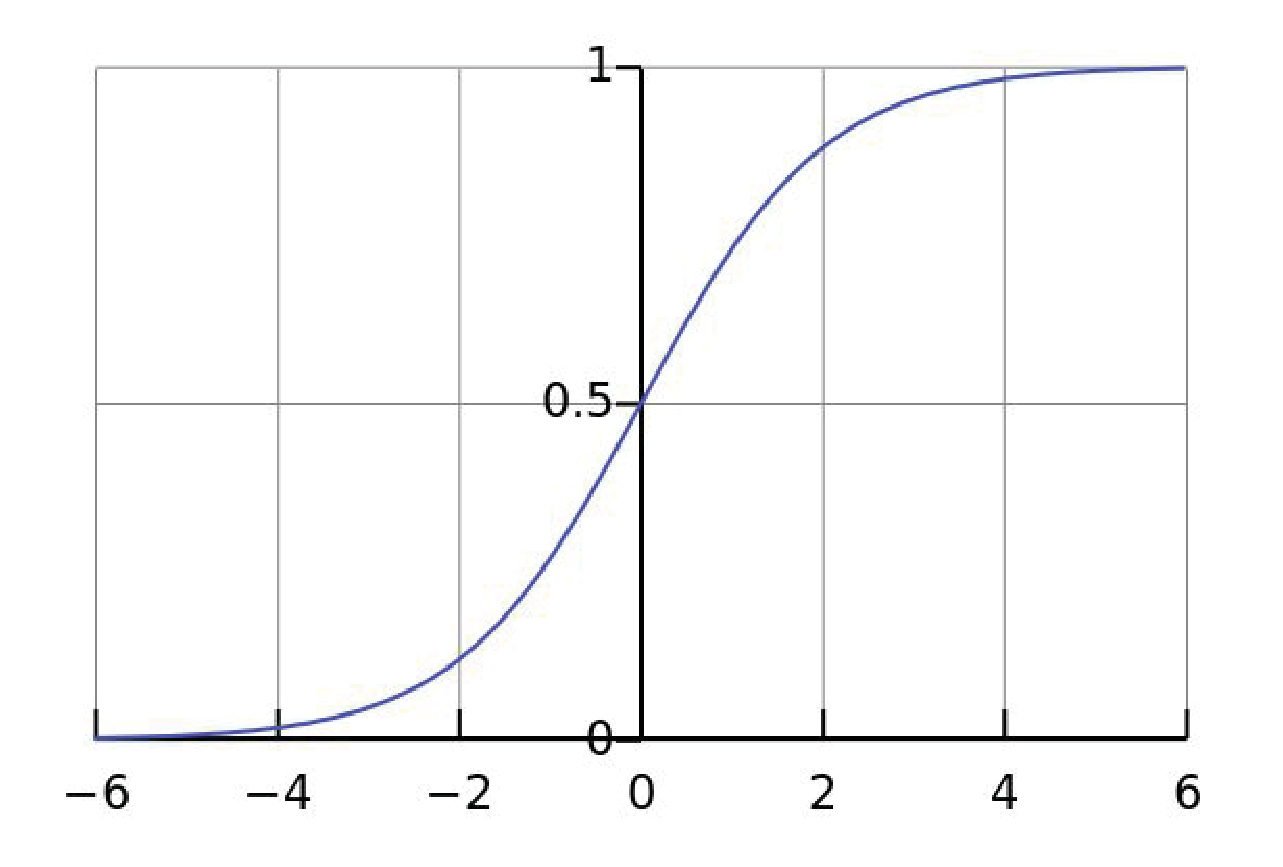
\includegraphics[width=0.55\textwidth]{logistics_function.eps}
  \caption{逻辑函数}
\end{figure}
\begin{figure}[!htb]
  \centering
  \includegraphics[width=0.6\textwidth]{1412.eps}
  \caption{线性可分模型构想}
\end{figure}

逻辑函数:$$y=h(z)=\frac{1}{1+exp(-z)}$$$$h_\theta(\theta^T x)=\frac{1}{1+exp(-\theta^Tx)}$$

易知:$$z>>0~,~y=1~~~~~~~~z<<0~,~y=0$$



反之:$$y=1~,~z>>0~~~~~~~~y=0~,~z<<0$$

那么试想若对于一个二分类问题,线性可分下最优的决策边界就是离两类数据特征向量\textbf{最远}的情况。这就是由逻辑回归以及事实情况启发而来,然后是要解决线性可分下找出这样的决策边界,即就是分割(超)平面。

那么从下面只有一两个特征线性可分的数据来看,这样的决策边界事实上只与少量的特征向量相关,就是离这个超平面最近的这几个点,把这些点称为\textbf{支持向量}。这也是支持向量机高效的原因。

那么接下来要做的工作便是利用数学方法将求出这个显然存在的分割最优超平面。为此定义了两种间隔,\textbf{函数间隔}(functional margin)与\textbf{几何间隔}(geometric margin)。

\subsubsection{函数间隔与几何间隔}
一般来说,一个点的离分离超平面的远近可用$~|w\cdot x+b|~$的大小来衡量,而分类的正确性可用$~(w\cdot x+b)~$与类标记~y~的符号是否一致来判定。所以可以用$~y(w\cdot x+b)~$来表示分类的正确性与确信度。这就是\textbf{函数间隔}。

\textbf{函数间隔} ~~对于给定的训练集数据集~T~和超平面$~(w,b)~$,~T~中所有的样本点$~(x_i,y_i)~$的函数间隔为
$$\hat{\gamma_i}=y_i(w\cdot x_i+b)$$

定义超平面$~(w,b)~$关于训练集~T~的函数间隔为超平面$~(w,b)~$关于~T~中所有样本点$~(x_i,y_i)~$的函数间隔之最小值,即
$$\hat{\gamma} = \min \limits_{i=1,...,N} \hat{\gamma_i}$$


函数间隔可以表示分类预测的正确性以及确信度,但是选择分离超平面时,只有函数间隔还不够。原因是如果成比例的改变~w,b~,超平面没有变而函数间隔为原来的二倍。因此我们需要规范化,如$~||w||=1~$,使得函数间隔变为\textbf{几何间隔}。

\textbf{几何间隔} ~~对于给定的数据集~T~和超平面$~(w,b)~$,定义超平面$~(w,b)~$关于样本点$~(x_i,y_i)~$的几何间隔为
$$\gamma_i = y_i(\frac{w}{||w||}\cdot x_i+\frac{b}{||w||})$$

定义超平面$~(w,b)~$关于训练集~T~的几何间隔为超平面$~(w,b)~$关于~T~中所有样本点$~(x_i,y_i)~$的几何间隔的最小值,即
$$\gamma = \min \limits_{i=1,...N} \gamma_i$$

\begin{figure}[!htb]
  \centering
  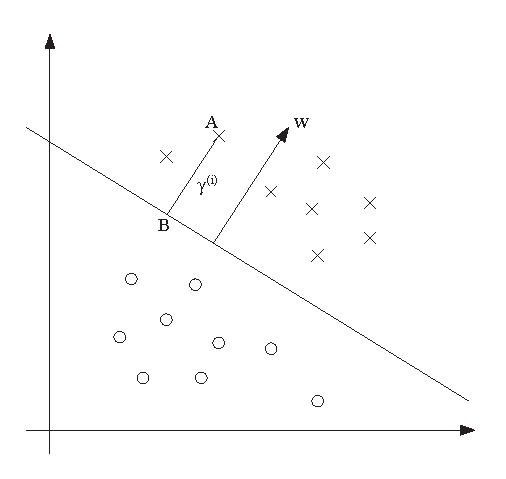
\includegraphics[width=0.45\textwidth]{geometric_margin.eps}
  \caption{几何间隔}
\end{figure}

\subsubsection{最优间隔分类器的产生}
定义了函数间隔与几何间隔之后,然后利用数学优化方法,显式表达这个求最优分割超平面的优化问题。

\textbf{优化问题的转变}
\begin{align}
            &\max \limits_{\gamma,w,b}~\gamma  \nonumber  \\
    s.t.~~  &y^{(i)}(w^Tx^{(i)}+b)~\geq~\gamma,~~i=1,...,m\nonumber\\
            &||w||=1   \nonumber
\end{align}

由于一号优化问题中$~||w||=1~$是一个非凸性的约束,导致此优化问题难以求解,因此改变这个优化问题。
\begin{align}
            &\max \limits_{\hat{\gamma,w,b}}~\frac{\hat{\gamma}}{||w||}  \nonumber  \\
    s.t.~~  &y^{(i)}(w^Tx^{(i)}+b)~\geq~\gamma,~~i=1,...,m \nonumber
\end{align}

二号优化问题用了另外的放缩方式,但依然是一个非凸性的优化问题,还需进行转变利用放缩条件$~\hat{\gamma}=1~$产生三号也是最终的优化问题。
\textcolor{red}{\begin{align}
            &\min \limits_{w,b} ~\frac{1}{2}||w||^2  \nonumber  \\
    s.t.~~  &y_i(w\cdot x_i+b)-1 \geq 0,~~i=1,2,...,m\nonumber
\end{align}}


\textbf{最大间隔分离超平面的存在唯一性定理}~~若训练集~T~线性可分,则可将训练数据集中的样本点完全正确分开的最大间隔分离超平面存在且唯一。

那么由定理可知最优间隔超平面存在且唯一,那么求解这个凸二次规划问题既可以产生这个最有间隔分类器。关于求解凸二次规划问题,可以利用如梯度下降等最优化算法下的QP软件来做,现在大多数是利用拉格朗日对偶学习算法来做。不仅是在求解速度上有优势,而且便于由线性向非线性扩充。

\textbf{支持向量与间隔边界} ~~ 在线性可分情况下,训练数据集的样本点中与分离超平面距离最近的样本点的实例称为支持向量(support vector), 支持向量是使约束条件式等号成立的点,即
$$y_i(w\cdot x_i+b)-1=0$$

\begin{figure}[!htb]
  \centering
  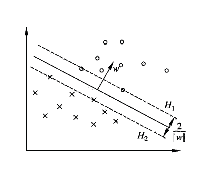
\includegraphics[width=0.45\textwidth]{support_vector.eps}
  \caption{支持向量机}
\end{figure}

注意到$~H_1~$和$~H_2~$平行,并且没有实例点落在它们中间,在$~H_1~$与$~H_2~$,之间形成一条长带,分离超平面与它们平行且位于它们中央长带的宽度,即$~H_1~$与$~H_2~$之间的距离称为间隔(margin)。间隔依赖于分离超平面的法向量~w~,等于$~\frac{2}{||w||}~$,$~H_1~$和$~H_2~$称为间隔边界。

在决定分离超平而时只有支持向量起作用,而其他实例点并不起作用如果移动支持向量将改变所求的解,但是如果在间隔边界以外移动其他实例点,甚至去掉这些点,则解是不会改变的。由于支持向量奄确定分离超平面中起着决定性作用,所以将这种分类模型称为支持向量机支持向量的个数 般很少,所以支持向量机由很少的“重要的”训练样本确定。

\subsubsection{拉格朗日对偶}
为了求解线性可分支持向量机的最优化问题,将它作为原始最优化问题,应用拉格朗日对偶性,通过求解对偶问题(duality problem)得到原始问题(primal problem)的最优解,这就是线性可分支持向量机的对偶算法(duality algorithm).这样做的优点,一是对偶问题往往更容易求解,二是自然引入核函数,进而推广到非线性分类问题.

\textbf{拉格朗日数乘的一般形式}
\\ \indent问题:
\begin{align}
            &\min \limits_w ~~f(w)   \nonumber \\
    s.t.~~  &g_i(w)\leq0,~~i=1,...,k\nonumber\\
            &h_i(w) = 0,~~i=1,...,l\nonumber
\end{align}

拉格朗日对偶:~Lagrangian~ 拉格朗日算子
$$L(w,\alpha,\beta)=f(w)+\sum_{i=1}^{k}\alpha_ig_i(w)+\sum_{i=1}^{l}\beta_ih_i(w)$$
\indent定义,
$$\Theta_p(w) = \max \limits_{\alpha,\beta,\alpha_i\geq0} L(w,\alpha,\beta)$$
\indent\textbf{原始问题}
$$p^*=\min \limits_w \max \limits_{\alpha,\beta,\alpha_i\geq0} L(w,\alpha,\beta) = \min\limits_w \Theta_p(w)$$
\indent若$~g_i(w)>0~$或者$~h_i(w)\neq 0~$,有
$$\Theta_p(w) = \max \limits_{\alpha,\beta,\alpha_i\geq0} f(w)+\sum_{i=1}^{k}\alpha_ig_i(w)+\sum_{i=1}^{l}\beta_ih_i(w)=\infty $$
\indent 否则:
$$\Theta_p(w) = f(w)$$
\indent 有,
\begin{equation}\nonumber
\Theta_p(w)=
\begin{cases}
f(w)& \text{w满足原始约束}\\
\infty&\text{w不满足原始约束}
\end{cases}
\end{equation}
\indent 最终导出
$$\min \limits_w \Theta(w) = \min \limits_w ~f(w)  ~~~s.t.~ ...$$

\textbf{对偶问题} ~~\\
\indent 定义
$$\Theta_D(\alpha,\beta)=\min \limits_w L(w,\alpha,\beta)$$
$$d^* = \max \limits_{\alpha\geq0,\beta} \min L(w,\alpha,\beta) = \max\limits_{\alpha\geq0,\beta} \Theta_D(\alpha,\beta)$$

\textbf{定理} ~~$d^* = \max \limits_{\alpha\geq0,\beta} \min L(w,\alpha,\beta)\leq \min \limits_w \max \limits_{\alpha,\beta,\alpha_i\geq0} L(w,\alpha,\beta) = p^*$ \\
\indent~~~~~~~~~~~~即就是:~~~~~~~~~~$d^*\leq p^*$

对于对偶问题有很多有用的性质;解决原始优化问题的有效途径就是解决对偶问题。那么等号在什么条件下成立,就是KKT条件。

\textbf{KKT条件}(对偶问题$~d^*~$与原始问题$~p^*~$等价条件)\\
$
\indent1.~~~\frac{\partial}{\partial w_i}L(w^*,\alpha^*,\beta^*) =0,~~i=1,...,n   \\
\indent2.~~~\frac{\partial}{\partial \beta_i}L(w^*,\alpha^*,\beta^*) =0,~~i=1,...,l  \\
\indent3.~~~\alpha_i^*g_i(w^*)=0,~~i=1,...,k\\
\indent4.~~~g_i(w^*)\leq0,~~i=1,...,k \\
\indent5.~~~\alpha_i\geq0,~~i=1,...,k
$

由3可知,~~~~~~~~当$~\alpha_i>0~$时,$g_i(w^*)=0$\\
\indent ~~~~~~~~~~~~~~~~~~~~~~~当$~\alpha_i\neq0~$时,$g_i(w^*)=0$

\subsubsection{利用对偶问题求解最优间隔分类器}
利用拉格朗日对偶求得原始问题的对偶问题,再解决对偶问题实现对原始问题的求解。这样做的好处是求解容易以及便于向非线性扩展。

\textbf{原始问题} ~~
\begin{align}
            &\min \limits_{w,b} ~\frac{1}{2}||w||^2  \nonumber  \\
    s.t.~  &y_i(w\cdot x_i+b)-1 \geq 0,~~i=1,2,...,m\nonumber
\end{align}
\indent\textbf{对偶问题} ~~
\begin{align}
   &L(w,b,\alpha) ~=~ \frac{1}{2}||w||^2-\sum_{i=1}^{m}\alpha_i~[y^{(i)}(w^Tx^{(i)}+b)-1] \nonumber\\
   &\theta_D(\alpha)~=~\min \limits_{w,b} L(w,b,\alpha)   \nonumber\\
   \text{求解:} &\textcircled{\footnotesize{1}} ~\text{先最小化lagrangian.$~L(w,b,\alpha)~$}  \nonumber\\
                &\nabla_wL(w,b,\alpha)=w-\sum_{i=1}^{m}\alpha_iy^{(i)}x^{(i)}=0 \nonumber\\
                &\textcolor{red}{w = \sum_{i=1}^{m}\alpha_iy^{(i)}x^{(i)}} \nonumber \\
                &\frac{\partial}{\partial b} L(w,b,\alpha) = \sum_{i=1}^{m}\alpha_iy^{(i)}=0 \nonumber\\
                &\textcolor{red}{\sum_{i=1}^{m}\alpha_iy^{(i)}=0} \nonumber \\
                &\textcircled{\footnotesize{2}} ~\text{代入到原式:}\nonumber\\
                &L(w,b,\alpha) \nonumber \\
                &=\frac{1}{2}||w||^2-\sum_{i=1}^{m}\alpha_i~[y^{(i)}(w^Tx^{(i)}+b)-1] \nonumber\\
                &=\frac{1}{2}ww^T-\sum_{i=1}^{m}\alpha_iy^{(i)}x^{(i)}w^T-\sum_{i=1}^{m}\alpha_iy^{(i)}b+\sum_{i=1}^{m}\alpha_i \nonumber \\
                &=\frac{1}{2}ww^T-ww^T-\sum_{i=1}^{m}\alpha_iy^{(i)}b+\sum_{i=1}^{m}\alpha_i \nonumber \\
                &=-\frac{1}{2}\sum_{i=1}^{m}\alpha_iy^{(i)}x^{(i)}(\sum_{j=1}^{m}\alpha_iy^{(j)}x^{(j)})^T-b\sum_{i=1}^{m}\alpha_iy^{(i)}+\sum_{i=1}^{m}\alpha_i \nonumber \\
                W(\alpha)&=\sum_{i=1}^{m}\alpha_i-\frac{1}{2}\sum_{i=1}^{m}\sum_{j=1}^{m}\alpha_i\alpha_jy^{(i)}y^{(j)}<x^{(i)},x^{(j)}> \nonumber
\end{align}

\indent得到最终的对偶优化问题:
\textcolor{red}{\begin{align}
            &\min \limits_\alpha ~~~\frac{1}{2}\sum_{i=1}^{m}\sum_{j=1}^{m}\alpha_i\alpha_jy^{(i)}y^{(j)}<x^{(i)},x^{(j)}>-\sum_{i=1}^{m}\alpha_i \nonumber\nonumber\\
         &~~~~~~~~~~~~~~~~~~~~s.t.~~\alpha_i\geq 0,~~i=1,...,m \nonumber \\
               &~~~~~~~~~~~~~~~~~~~~~~~~~~~\sum_{i=1}^{m}\alpha_iy^{(i)}=0 \nonumber
\end{align}}
\indent最终要解决此对偶问题,1998年John.C.platt发表了一篇论文~"Sequential Minimal Optimization:A Fast Algorithm For Training Support Vector Machines"~or SMO algorithm 很好的解决了这个优化问题。


\subsubsection{软间隔支持向量机}
在此之前所有的讨论都是建立在数据明显线性可分下进行的,接下来要介绍一种~SVM~的变化形式来解决允许少量错误分点的情况,就是引入~L1~范式的正则化项(松弛变量)。这样做的好处是防止模型过拟合,使模型更稳定。
\begin{figure}[!htb]
  \centering
  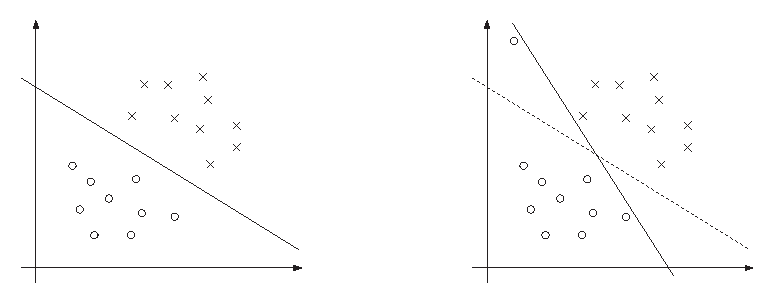
\includegraphics[width=0.78\textwidth]{soft.eps}
  \caption{软间隔支持向量机}
\end{figure}

\textbf{原始问题加入正则化项} ~~
\begin{align}
            &\min \limits_{w,b} ~\frac{1}{2}||w||^2 + C\sum_{i=1}^{m}\xi_i  \nonumber  \\
    s.t.~~  y_i(w\cdot& x_i+b) \geq 1-\xi_i,~~i=1,2,...,m\nonumber\\
            ~~~&\xi_i\geq 0,~~i=1,...,m. \nonumber
\end{align}

\textbf{得到对偶问题} ~~
\begin{align}
            &\min \limits_\alpha ~~~\frac{1}{2}\sum_{i=1}^{m}\sum_{j=1}^{m}\alpha_i\alpha_jy^{(i)}y^{(j)}<x^{(i)},x^{(j)}>-\sum_{i=1}^{m}\alpha_i \nonumber\nonumber\\
         &~~~~~~~~~~~~~~~~~~s.t.~~0 \leq\alpha_i\leq \textcolor{red}{C},~~i=1,...,m \nonumber \\
               &~~~~~~~~~~~~~~~~~~~~~~~~~~~\sum_{i=1}^{m}\alpha_iy^{(i)}=0 \nonumber
\end{align}

\textbf{由KKT条件可知}
\begin{align}
    \alpha_i=0 ~~~ \Rightarrow  &~~~y^{(i)}(w^Tx^{(i)}+b)\geq1   \nonumber\\
    \alpha_i=C ~~~ \Rightarrow &~~~y^{(i)}(w^Tx^{(i)}+b)\leq1   \nonumber\\
    0\leq\alpha_i\leq C ~~~ \Rightarrow &~~~y^{(i)}(w^Tx^{(i)}+b)=1   \nonumber
\end{align}

\subsubsection{引入核函数}
分类数据从线性可分,有少量早噪声点,我们可以利用~SVM~或者~SVM~的变形来解决;但大多数的分类数据是线性不可分的,此时我们就要引入核函数,利用核技巧来解决这一线性不可分的情况。

\begin{figure}[!htb]
  \centering
  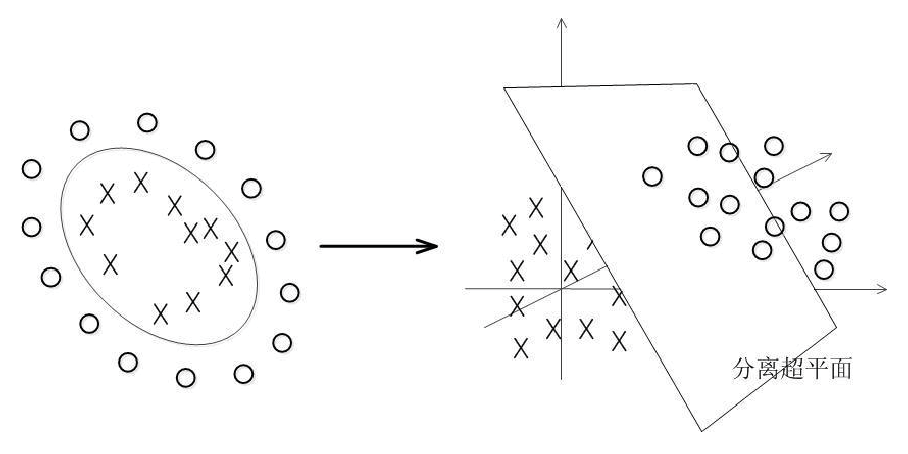
\includegraphics[width=0.72\textwidth]{kernel.eps}
  \caption{核技巧}
\end{figure}

\textbf{核} \\
\indent 特征映射~~feature~mapping.\\
\indent 一维特征$~x~\rightarrow~$三维特征$~\Phi(x)=\begin{bmatrix} x \\ x^2\\ x^3\end{bmatrix}~$\\
\indent利用特征映射来代替对偶问题中的内积,是一种好的方法,但是$~\Phi(x)~$一般维度很高甚至是无限维,这就导致利用$~<\Phi(x^{(i)}),\Phi(x^{(j)})>~$代替$~<x^{(i)},x^{(j)}>~$代价非常大。如此,便引入了核函数。

\textbf{核函数} \\
\indent举例,核函数及对应的核:
\begin{align}
    \textcircled{\footnotesize{1}}&~~x,z\in R^n \nonumber\\
    K(x,z) &~=~ (x^Tz)^2 \nonumber \\
           &~=~ (\sum_{i=1}^{n}x_iz_i)(\sum_{j=1}^{n}x_jz_j) \nonumber \\
           &~=~ \sum_{i,j=1}^{n}(x_ix_j)(z_iz_j) ~~~~~~~~~~~~~~\textcolor{red}{O(n)}\nonumber\\
           ~&~\nonumber\\
    \Phi(x)&~=~ \begin{bmatrix} x_1x_1 \\ x_1x_2\\ x_1x_3 \\ x_2x_1 \\ x_2x_2 \\ x_2x_3\\ x_3x_1 \\x_3x_2\\x_3x_3  \end{bmatrix}~~~~~~~~~~~~~~~~~~~~~~~~~~~\textcolor{red}{O(n^2)}\nonumber\\
         ~&~    \nonumber\\
    \textcircled{\footnotesize{2}}&~~K(x,z)=(x^Tz+c)^d ~~~~~~~~~~\textcolor{red}{O(n)}  \nonumber\\
    ~&~~\Phi(x)~ \text{的维度与的相关。 }~~~~\textcolor{red}{O(n^d)} \nonumber \\
    ~&~    \nonumber\\
    \textcircled{\footnotesize{3}}&~~\text{径向基函数(radial basis function)} \nonumber \\
    K(x,y) &~=~\exp\Big(\frac{-||x-y||^2}{2\sigma^2}\Big) ~~~~~~~~~~\textcolor{red}{O(n)} \nonumber \\
    ~&~~\Phi(x)~ \text{无限维}~~~~~~~~~~~~~~~~~~~~~~~~~\textcolor{red}{O(\infty)} \nonumber
\end{align}
\indent 事实上,对于任意给定的核函数,是否一定存在原始的核,答案显然是不一定的。那其中的关系由~Mercer~定理给出。

\textbf{Mercer~定理}~~\textcolor{red}{任何半正定对称函数都可以作为核函数。}\\
\indent K~是一个~Mercer~核,其充要条件是$~\{x^{(1)},x^{(2)},...,x^{(m)}\}~$所对应的核矩阵是对称半正定矩阵。

\textbf{引入高斯核得到新的对偶优化问题}
\begin{align}
            &\min \limits_\alpha ~~~\frac{1}{2}\sum_{i=1}^{m}\sum_{j=1}^{m}\alpha_i\alpha_jy^{(i)}y^{(j)}\textcolor{red}{K<x^{(i)},x^{(j)}>}-\sum_{i=1}^{m}\alpha_i \nonumber\nonumber\\
         &~~~~~~~~~~~~~~~~~~s.t.~~0 \leq\alpha_i\leq \textcolor{red}{C},~~i=1,...,m \nonumber \\
               &~~~~~~~~~~~~~~~~~~~~~~~~~~~\sum_{i=1}^{m}\alpha_iy^{(i)}=0 \nonumber \\
               ~&~ \nonumber\\
               &\text{得到}~,\alpha^*,w^* ~,~ b^* \nonumber\\
               &\text{构造决策函数:}~f(x)~=~sign~\Big(\sum_{i=1}^{m}~\alpha^*_iy_iK(x,x_i)+b^*\Big) \nonumber
\end{align}
\indent最终的问题在于如何求得最终优化问题的最优解,这便是利用~SMO~算法。

\subsubsection{SMO~算法}
SOM~算法全称~Sequential~Minimal~Optimization.~是1998年4月~John.C.platt~发表的关于训练支持向量机一种快速的算法。它相较于其他训练支持向量机的算法有明显的速度优势。它的灵感来源于坐标上升算法~(Coordinate~ascent)~.

\textbf{坐标上升}\\
$
\indent Repeat\{\\
\indent~~~~~~~~    for ~i=1 ~to~ m\{\\
\indent~~~~~~~~~~~~~~~~        \alpha_i :=arg~ \max \limits_{\alpha_i}~W(\alpha_1,..,\alpha_{i-1},\alpha_i,\alpha_{i+1},...,\alpha_m)\\
\indent~~~~~~~~    \}\\
\indent\}
$
\begin{figure}[!h]
\begin{minipage}
{0.5\linewidth}
\centering
\includegraphics[width=2.22in]{Gradient_descent.eps}
\caption{梯度下降}
\end{minipage}
%
\begin{minipage}
{0.5\linewidth}
\centering
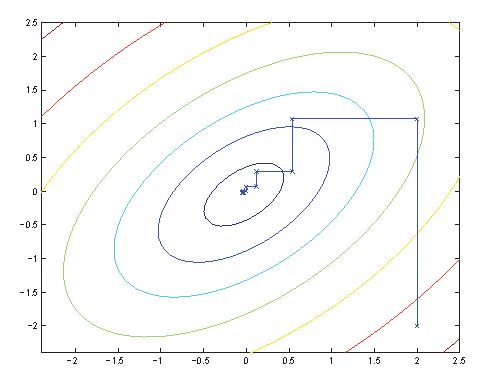
\includegraphics[width=2.22in]{Coordinate_ascent.eps}
\caption{坐标上升}
\end{minipage}
\end{figure}

\indent 坐标上升相较于其他最优化算法,如牛顿法来讲,是一种“曲线救国”的形式。虽然它收敛时的迭代次数要远多于牛顿法,但是对于单变量的优化问题它拥有明确的解析解,它的执行速度是非常快的。

\indent 利用坐标上升的思想来解决支持向量机的对偶问题就是SMO算法的实质,但是坐标上升的基本形式不能直接用于~SVM~的对偶优化问题,应为它有一个关于$~\alpha~$的等式约束。所以~SMO~算法每次优两个$~\alpha~$变量。

\textbf{SMO~算法框架}~~\\
\indent 框架:\\
\indent ~~~~~~~~~~选择$~\alpha_i,\alpha_j~$。(经验法则亦或者是启发式方法)\\
\indent ~~~~~~~~~~固定其他所有$~\alpha_i~$。\\
\indent ~~~~~~~~~~同时使得$~\alpha_i,\alpha_j~$最优。\textcolor{red}{(核心步骤)}

\textbf{核心步骤的数学推导}~~\\
\indent 对偶优化问题:
\begin{align}
            &\min \limits_\alpha ~~~\frac{1}{2}\sum_{i=1}^{m}\sum_{j=1}^{m}\alpha_i\alpha_jy^{(i)}y^{(j)}\textcolor{red}{K<x^{(i)},x^{(j)}>}-\sum_{i=1}^{m}\alpha_i \nonumber\nonumber\\
         &~~~~~~~~~~~~~~~~~~s.t.~~0 \leq\alpha_i\leq \textcolor{red}{C},~~i=1,...,m \nonumber \\
               &~~~~~~~~~~~~~~~~~~~~~~~~~~~\sum_{i=1}^{m}\alpha_iy^{(i)}=0 \nonumber
\end{align}

\indent 依据坐标上升思想,控制变量剩两个得到新的优化问题:~~
\begin{align}
    &~~~~~~~~~~~~~~~~~~~~~\min \limits_{\alpha_1,\alpha_2} \Psi (\alpha_1,\alpha_2) \nonumber \\
    &~~~~~~~~~~~~~~~~=\min \limits_{\alpha_1,\alpha_2}\frac{1}{2}K_{11}\alpha_1^2+\frac{1}{2}K_{22}\alpha_2^2+y_1y_2\alpha_1\alpha_2 \nonumber \\
    &~~~~~~~~~~~~~~~~~~~~~~~~~~~~~~~~~-(\alpha_1+\alpha_2)+y_1v_1\alpha_1+y_2v_2\alpha_2+Constant   \tag{1}  \\
    &~~~~~~~~~~~~~~~~~~~~~~~~~~~ v_i = \sum_{j=3}^{m} \alpha_i\alpha_jK(x_i,x_j) \nonumber \\
    &~~~~~~~~~~~~~~~~~~~~~~~~~~~~s.t.~~~0\leq\alpha_1,\alpha_2 \leq C \nonumber \\
    &~~~~~~~~~~~~~~~~~~~~~~~~~\alpha_1y_1+\alpha_2y_2 = -\sum_{i=3}^{m}\alpha_iy_i =\xi \nonumber \\
    &~~~~~~~~~~~~~~~~\Rightarrow~~\alpha_1=(\xi-\alpha_2y_2)y_1   \tag{2}
\end{align}
\indent 将(2)代入(1)得到一元二次函数的优化问题:
\begin{align}
    &~~~~~~~~~~~~~~~~\min \limits_{\alpha_2}\phi(\alpha2)=\frac{1}{2}K_{11}((\xi-\alpha_2y_2)y_1)^2+\frac{1}{2}K_{22}\alpha_2^2+y_1y_2(\xi-\alpha_2y_2)y_1\alpha_2 \nonumber \\
    &~~~~~~~~~~~~~~~~~~~~~~~~-((\xi-\alpha_2y_2)y_1+\alpha_2)+y_1v_1(\xi-\alpha_2y_2)y_1+y_2v_2\alpha_2+Constant
\end{align}
\indent 利用微分求这个最小化问题的最优解:
 \begin{align}
    &\frac{\partial\phi(\alpha_2)}{\partial\alpha_2}=(K_{11}+K_{22}-K_{12})\alpha_2-K_{11}\xi y_2 \nonumber \\
    &~~~~~~~~~~~~~~~~~+K_{11}\xi y_2+y_1y_2-1-v_1y_2+v_2y_1=0    \nonumber \\
    &~~~~~~\text{令求得的$~\alpha_1,\alpha_2~$为$~\alpha_1^{new},\alpha_2^{new}~$}. ~~~~~~\text{未更新的$~\alpha_1,\alpha_2~$为$~\alpha_1^{old},\alpha_2^{old}~$}. \nonumber \\
    &\text{由于等式约束条件$~\sum_{i=1}^{m}y^{(i)}\alpha_i=0~$有:} \nonumber \\
    &\alpha_1^{old}y_1+\alpha_2^{old}y_2 = -\sum_{i=3}^{m}\alpha_iy_i =\xi=\alpha_1^{new}y_1+\alpha_2^{new}y_2 \nonumber \\
    &~~~~~~~~~~~~~~~~~\Rightarrow\xi = \alpha_1^{old}y_1+\alpha_2^{old}y_2  \\
    &\text{真实值与预测值之间的误差:} \nonumber\\
    &~~~~~~~~~~~~~~~~~~~~~~~E_i = f(x_i)-y_i \\
    &~~~~~~~~~~~~~~~~~~~~~~~f(x)=\sum_{i=1}^{N}\alpha_iy_iK(x_i,x)+b   \nonumber \\
    &~~~~~~\text{由于}~v_i = \sum_{j=3}^{m} \alpha_i\alpha_jK(x_i,x_j)~\text{因此:} \nonumber \\
    &~~~~~~~~~~~~~~~~~~~~~~~v_1=f(x_1)-\sum_{j=1}^{2}\alpha_jy_jK_{1j}-b \\
    &~~~~~~~~~~~~~~~~~~~~~~~v_2=f(x_2)-\sum_{j=1}^{2}\alpha_jy_jK_{2j}-b \\
    &\text{将(4)(6)(7)代入求导式:}  \nonumber \\
    &~~~~~~(K_{11}+K_{22}-2K_{12})\alpha_2-(\alpha_1^{old}y_1+\alpha_2^{old}y_2)y_2(K_{11}-K_{22})+y_1y_2-y_2^2 \nonumber\\
    &~~~~~~~~~~+y_2(f(x_2)-f(x_1)+\alpha_1^{old}y_1k_{11}+\alpha_2^{old}y_2K_{12}-\alpha_1^{old}y_1K_{12}-\alpha_2^{old}y_2K_{22})=0 \nonumber \\
    &\Rightarrow(K_{11}+K_{22}-2K_{12})\alpha_2=\alpha_2^{old}(K_{11}+K_{22}-2K_{12})+y_2(f(x_1)-f(x_2)-y_1+y_2) \nonumber \\
    &~~~~~~\text{令}~\eta=(K_{11}+K_{22}-2K_{12})=||\phi(x_1)-\phi(x_2)||^2 \nonumber \\
    &\Rightarrow\textcolor{red}{ \alpha_2^{new,unclipped}=\alpha_2^{old}+\frac{y_2(E_1-E_2)}{\eta}}
\end{align}
\indent由于求得的$~\alpha_2^{new,unclipped}~$是未利用不等式约束的解析解,我们进一步依据不等式约束$~0\leq \alpha_{1,2}\leq C~$和等式$~\alpha_1^{new}y_1+\alpha_2^{new}y_2  =\xi~$来进行裁剪,使求得的$~\alpha_{1,2}~$都满足约束。

裁剪~~情况1:
\begin{align}
    &y_1\neq y_2 ~\Rightarrow~\alpha_1-\alpha_2 = K   \nonumber \\
    &L=\max(0,-K)=\max(0,\alpha_2^{old}-\alpha_1^{old}) \nonumber\\
    &H=\min(0,C-K)=\min(0,C+\alpha_2^{old}-\alpha_1^{old}) \nonumber
\end{align}
\begin{figure}[!htb]
  \centering
  \includegraphics[width=0.8\textwidth]{clipped.eps}
  \caption{裁剪}
\end{figure}
\indent~~~~~~~~~~情况2:
\begin{align}
    &y_1= y_2 ~\Rightarrow~\alpha_1+\alpha_2 = k   \nonumber \\
    &L=\max(0,K-C)=\max(0,\alpha_2^{old}+\alpha_1^{old}-C) \nonumber\\
    &H=\min(K,C)=\min(0,c+\alpha_2^{old}-\alpha_1^{old}) \nonumber
\end{align}
\indent 裁剪后:
\textcolor{red}{\begin{equation}\nonumber
\alpha_2^{new,clipped}=
\begin{cases}
H& ,\alpha_2^{new,unclipped}>H\\
\alpha_2^{new,unclipped}&,L\leq \alpha_2^{new,unclipped}\leq H\\
L&,\alpha_2^{new,unclipped}>L
\end{cases}
\end{equation}}

求解$~\alpha_1~$:
\begin{align}
  &\alpha_1^{old}y_1+\alpha_2^{old}y_2=\alpha_1^{new}y_1+\alpha_2^{new}y_2 \nonumber\\
  &\textcolor{red}{\alpha_1^{new}=\alpha_1^{old}+y_1y_2(\alpha_2^{old}-\alpha_2^{new})}
\end{align}

\textcolor{red}{特殊情况:\textcircled{\footnotesize{1}}$~\eta<0~$,核矩阵为非半正定矩阵。\\
\indent~~~~~~~~~~~~~~~~~~~~\textcircled{\footnotesize{2}}$~\eta=0~$,样本$~x_1,x_2~$输入特征相同。\\
\indent~~~~~~~~~~~~~~~$~\Rightarrow$这两种情况下,都是在边界上取得极值。}
\begin{align}
  &~~~~~~\text{则将}~~~\alpha_2^{new}=L~,~\alpha_2^{new}=H \nonumber \\
  &~~~~~~\text{代入(9)式得}~~~\alpha_1^{new}=L_1~,~\alpha_1^{new}=H_1~,~s=y_1y_2. \nonumber \\
  &~~~~~\Rightarrow L_1=\alpha_1^{old}+s(\alpha_2^{old}-L) \nonumber \\
  &~~~~~~~~~~~H_1=\alpha_1^{old}+s(\alpha_2^{old}-H) \nonumber \\
  &~~~~~~\text{将代入(1)式中比较$~\Psi(\alpha_1=L_1,\alpha_2=L)~$与$~\Psi(\alpha_1=H_1,\alpha_2=H)~$取小得特殊情况的解析解。} \nonumber
\end{align}
\begin{align}
  \Psi_L&=\Psi(L_1,L)=\Psi(\alpha_1=L_1,\alpha_2=L)    \nonumber\\
        &=\frac{1}{2}L_1^2K_{11}+\frac{1}{2}L_2^2K_{22}+sK_{12}LL_1-(L_1+L)+y_1v_1L_1+y_2v_2L_2+Constant \nonumber \\
        &=...+L_1(y_1v_1-1)+L_2(y_2v_2-1)+Constant \nonumber \\
        &=...+L_1(y_1[f(x_1)-\alpha_1y_1K_{11}-\alpha_2y_2K_{12}-b]-1)+L_2(y_2v_2-1)+Constant \nonumber \\
        &=...+L_1([f(x_1)-y_1+y_1-b-\alpha_1y_1K_{11}-\alpha_2y_2K_{12}]-1)+L_2(y_2v_2-1)+Constant \nonumber \\
        &=...+L_1(y_1(E_1-b)+1-\alpha_1K_{11}-y_1y_2K_{12}\alpha_2-1)+L_2(y_2v_2-1)+Constant \nonumber \\
        &=\frac{1}{2}L_1^2K_{11}+\frac{1}{2}L_2^2K_{22}+sK_{12}LL_1+L_1f_1+L_2f_2+Constant \nonumber \\
        &~~~~~~~~~~~~f_1=y_1(E_1-b)-\alpha_1K_{11}-y_1y_2\alpha_2K_{12} \nonumber \\
        &~~~~~~~~~~~~f_2=y_2(E_2-b)-\alpha_2K_{22}-y_1y_2\alpha_1K_{12} \nonumber \\
  \Psi_H&=\Psi(H_1,H)=\Psi(\alpha_1=H_1,\alpha_2=H)    \nonumber\\
        &=\frac{1}{2}H_1^2K_{11}+\frac{1}{2}H_2^2K_{22}+sK_{12}HH_1+H_1f_1+H_2f_2+Constant \nonumber
\end{align}

\textcolor{red}{计算阈值~b~和差值$~E_i~$}
\begin{align}
   &\textcircled{\footnotesize{1}}  ~ \text{若}~~~0<\alpha_1^{new}<C~,~\alpha_2^{new}=0~or~C \Rightarrow \sum_{i=1}^{N}\alpha_iy_iK_{i1}+b=y_1   \nonumber \\
   &~~~~~~~~~~\Rightarrow b_1^{new}=y_1-\sum_{i=3}^{m}\alpha_iy_iK_{i1}-\alpha_1^{new}y_1K_{11}-\alpha_2^{new}y_2K_{21}   \nonumber \\
   &~~~~~~~~~~~\text{因} ~ E_1=f(x_1)-y_1=\sum_{i=3}^{m}\alpha_iy_1K_{i1}+\alpha_1^{old}y_1K_{11}+\alpha_2^{old}y_2K_{21}+b^{old}-y_1\nonumber\\
   &~~~~~~~~~~\Rightarrow b^{new}=b_1^{new}=-E_1-y_1K_{11}(\alpha_1^{new}-\alpha_1^{old})-y_2K_{21}(\alpha_2^{new}-\alpha_2^{old})+b^{old}   \nonumber \\
   &\textcircled{\footnotesize{2}}      ~ \text{同理}~~~0<\alpha_2^{new}<C~,~\alpha_1^{new}=0~or~C \nonumber \\
   &~~~~~~~~~~\Rightarrow b^{new}=b_2^{new}=-E_2-y_1K_{12}(\alpha_1^{new}-\alpha_1^{old})-y_2K_{22}(\alpha_2^{new}-\alpha_2^{old})+b^{old}   \nonumber \\
   &\textcircled{\footnotesize{3}}   ~ \text{若}~~~0<\alpha_1^{new}<C~,~0<\alpha_2^{new}<C \Rightarrow  b^{new}=b_1^{new}=b_2^{new}   \nonumber \\
   &\textcircled{\footnotesize{4}}  ~ \text{若}~~~\alpha_1^{new}=0~or~C ,~\alpha_2^{new}=0~or~C \Rightarrow b^{new}=\frac{1}{2}(b_1^{new}+b_2^{new})     \nonumber
\end{align}

\textcolor{red}{变量的选取方法}\\
\indent SMO~算法在每个子问题中选择两个变量优化, 其中至少一个变量是违反 KKT条件的。\\
\indent\textcircled{\footnotesize{1}}第一个变量的选取方法:~~\\
\indent SMO~称选择第1个变量的过程为外层循环外层循环在训练样本中选取违反~KKT~条件最严重的样本点,并将其对应的变量作为第 1个变量.具体地,检验训练样本点$~(x_i,y_i)~$是否满足~KKT~条件 , 即
\\
~\\
\begin{align}
    \alpha_i=0 ~~~ \Leftrightarrow  &~~~y_ig(x_i)\geq1   \nonumber\\
    \alpha_i=C ~~~ \Leftrightarrow &~~~y_ig(x_i)\leq1   \nonumber\\
    0\leq\alpha_i\leq C ~~~ \Leftrightarrow &~~~y_ig(x_i)=1   \nonumber
\end{align}
其中,$~g(x_i)=\sum_{j=1}^{m}\alpha_jy_jK(x_i,x_j)+b~$.\\
\indent该检验是在$~\epsilon~$范围内进行的。在检验过程中,外层循环首先遍历所有满足条件$~0<\alpha_i<C~$的样本点,即在间隔边界上的支持向盘点,检验它们是否满足~KKT~条件如果这些样本点都满足~KKT~条件,那么遍历整个训练集,检验它们是否满足~KKT~条件.

\textcircled{\footnotesize{2}}第2个变量的选择 \\
\indent SMO~称选择第2个变量的过程为内层循环。假设在外层循环中已经找到第1个变量叫$~\alpha_1~$,现在要在内层循环中找第2个变量$~\alpha_2~$第2个变量选择的标准是希望能使$~\alpha_2~$有足够大的变化。\\
\indent由式(8)可知,$~\alpha_2^{new}~$是依赖于$~|E_1-E_2|~$的,为了加快计算速 ,一种简单的做法是选择$~\alpha_2~$,使其对应的$~|E_1-E_2|~$最大。因为$~\alpha_1~$已定,$~E_1~$也就确定了。如果$~E_1~$是正的,那么选择最小的$~E_i~$作为$~E_2~$,如果$~E_i~$是负的,那么选择最大的$~E_i~$作为$~E_2~$,为了节省计算时间,将所有$~E_i~$保存在一个列表中。\\
\indent在特殊情况下,如果内层循环通过以上方法选择的$~\alpha_2~$不能使目标函数有足够的下降,那么采用以下启发式规则继续选择$~\alpha_2~$·遍历在间隔边界上的支持向量点,依次将其对应的变量作为$~\alpha_2~$试用,直到目标函数有足够的下降若找不到合适的$~\alpha_2~$那么遍历训练数据集;若仍找不到合适的$~\alpha_2~$,则放弃第1个$~\alpha_1~$,再通过外层寻找$~\alpha_1~$。
\subsubsection{实战:简化版的SMO算法处理小规模数据集}
支持向量机优缺点\\
\textcolor{red}{优点}:泛化错误率低,计算开销不大,结果易解释。\\
\textcolor{red}{缺点}:泛化错误率低,计算开销不大,结果易解释。\\
适用数据类型:数值型和标称型数据。

SVM的一般流程\\
(1) 收集数据:可以使用任意方法。 \\
(2) 准备数据:需要数值型数据。\\
(3) 分析数据:有助于可视化分隔超平面。\\
(4) 训练算法:SVM的大部分时间都源自训练,该过程主要实现两个参数的调优。\\
(5) 测试算法:十分简单的计算过程就可以实现。\\
(6) 使用算法:几乎所有分类问题都可以使用SVM,值得一提的是,SVM本身是一个二类
分类器,对多类问题应用SVM需要对代码做一些修改。\\

\noindent程序核心函数代码:
\begin{lstlisting}
def selectJrand(i,m):
    j=i #we want to select any J not equal to i
    while (j==i):
        j = int(np.random.uniform(0,m))
    return j

def clipAlpha(aj,H,L):  #s.t. 0<=\alpha<=C
    if aj > H:
        aj = H
    if L > aj:
        aj = L
    return aj

def smoSimple(dataMatIn, classLabels, C, toler, maxIter):
    dataMatrix = np.mat(dataMatIn); labelMat = np.mat(classLabels).transpose()
    b = 0; m,n = np.shape(dataMatrix)
    alphas = np.mat(np.zeros((m,1)))
    iter = 0
    while (iter < maxIter):
        alphaPairsChanged = 0
        for i in range(m):
            fXi = float(np.multiply(alphas,labelMat).T\
            *(dataMatrix*dataMatrix[i,:].T)) + b
            Ei = fXi - float(labelMat[i])
            #if checks if an example violates KKT conditions
            if ((labelMat[i]*Ei < -toler) and (alphas[i] < C))
            or ((labelMat[i]*Ei > toler) and (alphas[i] > 0)):
                j = selectJrand(i,m)
                print("i",i,alphas[i])
                print("j",j,alphas[j])
                fXj = float(np.multiply(alphas,labelMat).T*\
                (dataMatrix*dataMatrix[j,:].T)) + b
                Ej = fXj - float(labelMat[j])
                alphaIold = alphas[i].copy(); alphaJold = alphas[j].copy();
                if (labelMat[i] != labelMat[j]):
                    L = max(0, alphas[j] - alphas[i])
                    H = min(C, C + alphas[j] - alphas[i])
                else:
                    L = max(0, alphas[j] + alphas[i] - C)
                    H = min(C, alphas[j] + alphas[i])
                if L==H: print ("L==H"); continue
                eta = 2.0 * dataMatrix[i,:]*dataMatrix[j,:].T -\
                dataMatrix[i,:]*dataMatrix[i,:].T - dataMatrix[j,:]*dataMatrix[j,:].T
                if eta >= 0: print ("eta>=0"); continue
                alphas[j] -= labelMat[j]*(Ei - Ej)/eta
                alphas[j] = clipAlpha(alphas[j],H,L)
                if (abs(alphas[j] - alphaJold) < 0.00001):
                    print ("j not moving enough",alphas[j])
                    continue
                alphas[i] += labelMat[j]*labelMat[i]*(alphaJold - alphas[j])
                print("i",i,alphas[i])
                print("j",j,alphas[j]);
                #update i by the same amount as j
                #the update is in the oppostie direction
                b1 = b - Ei- labelMat[i]*(alphas[i]-alphaIold)\
                *dataMatrix[i,:]*dataMatrix[i,:].T-labelMat[j]\
                *(alphas[j]-alphaJold)*dataMatrix[i,:]*dataMatrix[j,:].T
                b2 = b - Ej- labelMat[i]*(alphas[i]-alphaIold)\
                *dataMatrix[i,:]*dataMatrix[j,:].T-labelMat[j]\
                *(alphas[j]-alphaJold)*dataMatrix[j,:]*dataMatrix[j,:].T
                if (0 < alphas[i]) and (C > alphas[i]): b = b1
                elif (0 < alphas[j]) and (C > alphas[j]): b = b2
                else: b = (b1 + b2)/2.0
                alphaPairsChanged += 1
                print ("iter: %d i:%d, pairs changed %d" % (iter,i,alphaPairsChanged))
        if (alphaPairsChanged == 0): iter += 1
        else: iter = 0
        print ("iteration number: %d" % iter)
    return b,alphas

def test():
    dataArr,labelArr = svmMLiA.loadDataSet('testSet.txt')
    b,alpha = svmMLiA.smoSimple(dataArr,labelArr,0.6,0.001,80)
    print (b)
    print (alpha[alpha>0])
    for i in range(100):
        if alpha[i]>0.0:
            print (i,dataArr[i],labelArr[i])

\end{lstlisting}

\noindent实验结果运行时间:
\begin{lstlisting}
Time For Run SMO:15.935288698252556s
\end{lstlisting}

\noindent运行结果可视化图:
\begin{figure}[!htb]
  \centering
  \includegraphics[width=0.65\textwidth]{SMOSimple.eps}
  \caption{简化版~SMO~算法运行结果图}
\end{figure}

\noindent简化版的~SMO~算法:\\
\textcircled{\footnotesize{1}}  ~ 应用简化版的~SMO~算法来处理小规模数据集,不注重它的运行效率。       \\
\textcircled{\footnotesize{2}}  ~$~\alpha~$对选取比较粗糙,这是效率低下的主要原因。       \\
\textcircled{\footnotesize{3}}  ~不考虑$~\eta=(K_{11}+K_{22}-2K_{12})\leq0~$情况,事实上,这对算法的收敛没有太大影响。        \\
\textcircled{\footnotesize{4}}  ~没有向线性不可分的情况拓展,即就是没有使用核技巧,难以应用在实际中。        \\





\subsubsection{实战:完整版的SMO算法加速优化}
\noindent程序核心函数代码:
\begin{lstlisting}
class optStruct:
    def __init__(self,dataMatIn, classLabels, C, toler):  # Initialize the structure with the parameters
        self.X = dataMatIn
        self.labelMat = classLabels
        self.C = C
        self.tol = toler
        self.m = np.shape(dataMatIn)[0]
        self.alphas = np.mat(np.zeros((self.m,1)))
        self.b = 0
        self.eCache = np.mat(np.zeros((self.m,2))) #first column is valid flag

def calcEk(oS, k):
    fXk = float(np.multiply(oS.alphas,oS.labelMat).T*(oS.X*oS.X[k,:].T)) + oS.b
    Ek = fXk - float(oS.labelMat[k])
    return Ek

def selectJrand(i,m):
    j=i #we want to select any J not equal to i
    while (j==i):
        j = int(np.random.uniform(0,m))
    return j

def clipAlpha(aj,H,L):
    if aj > H:
        aj = H
    if L > aj:
        aj = L
    return aj

def selectJ(i, oS, Ei):         #this is the second choice -heurstic, and calcs Ej
    maxK = -1; maxDeltaE = 0; Ej = 0
    oS.eCache[i] = [1,Ei]  #set valid #choose the alpha that gives the maximum delta E
    validEcacheList = np.nonzero(oS.eCache[:,0].A)[0];print("the length of validEcacheList",len(validEcacheList))
    if (len(validEcacheList)) > 1:
        for k in validEcacheList:   #loop through valid Ecache values and find the one that maximizes delta E
            if k == i: continue #don't calc for i, waste of time
            Ek = calcEk(oS, k)
            deltaE = abs(Ei - Ek)
            if (deltaE > maxDeltaE):
                maxK = k; maxDeltaE = deltaE; Ej = Ek
        return maxK, Ej
    else:   #in this case (first time around) we don't have any valid eCache values
        j = selectJrand(i, oS.m)
        Ej = calcEk(oS, j)
    return j, Ej

def updateEk(oS, k):#after any alpha has changed update the new value in the cache
    Ek = calcEk(oS, k)
    oS.eCache[k] = [1,Ek]

def innerL(i, oS):
    Ei = calcEk(oS, i)
    if ((oS.labelMat[i]*Ei < -oS.tol) and (oS.alphas[i] < oS.C)) or ((oS.labelMat[i]*Ei > oS.tol) and (oS.alphas[i] > 0)):
        j,Ej = selectJ(i, oS, Ei) #this has been changed from selectJrand
        alphaIold = oS.alphas[i].copy(); alphaJold = oS.alphas[j].copy();
        if (oS.labelMat[i] != oS.labelMat[j]):
            L = max(0, oS.alphas[j] - oS.alphas[i])
            H = min(oS.C, oS.C + oS.alphas[j] - oS.alphas[i])
        else:
            L = max(0, oS.alphas[j] + oS.alphas[i] - oS.C)
            H = min(oS.C, oS.alphas[j] + oS.alphas[i])
        if L==H: print ("L==H"); return 0
        eta = 2.0 * oS.X[i,:]*oS.X[j,:].T - oS.X[i,:]*oS.X[i,:].T - oS.X[j,:]*oS.X[j,:].T
        if eta >= 0: print ("eta>=0"); return 0
        oS.alphas[j] -= oS.labelMat[j]*(Ei - Ej)/eta
        oS.alphas[j] = clipAlpha(oS.alphas[j],H,L)
        updateEk(oS, j) #added this for the Ecache
        if (abs(oS.alphas[j] - alphaJold) < 0.00001): print ("j not moving enough"); return 0
        oS.alphas[i] += oS.labelMat[j]*oS.labelMat[i]*(alphaJold - oS.alphas[j])#update i by the same amount as j
        updateEk(oS, i) #added this for the Ecache                    #the update is in the oppostie direction
        b1 = oS.b - Ei- oS.labelMat[i]*(oS.alphas[i]-alphaIold)*oS.X[i,:]*oS.X[i,:].T - oS.labelMat[j]*(oS.alphas[j]-alphaJold)*oS.X[i,:]*oS.X[j,:].T
        b2 = oS.b - Ej- oS.labelMat[i]*(oS.alphas[i]-alphaIold)*oS.X[i,:]*oS.X[j,:].T - oS.labelMat[j]*(oS.alphas[j]-alphaJold)*oS.X[j,:]*oS.X[j,:].T
        if (0 < oS.alphas[i]) and (oS.C > oS.alphas[i]): oS.b = b1
        elif (0 < oS.alphas[j]) and (oS.C > oS.alphas[j]): oS.b = b2
        else: oS.b = (b1 + b2)/2.0
        return 1
    else: return 0

def smoP(dataMatIn, classLabels, C, toler, maxIter):    #full Platt SMO
    oS = optStruct(np.mat(dataMatIn),np.mat(classLabels).transpose(),C,toler)
    iter = 0
    entireSet = True; alphaPairsChanged = 0
    while (iter < maxIter) and ((alphaPairsChanged > 0) or (entireSet)):
        alphaPairsChanged = 0
        if entireSet:   #go over all
            for i in range(oS.m):
                alphaPairsChanged += innerL(i,oS)
                print ("fullSet, iter: %d i:%d, pairs changed %d" % (iter,i,alphaPairsChanged))
            iter += 1
        else:#go over non-bound (railed) alphas
            nonBoundIs = np.nonzero((oS.alphas.A > 0) * (oS.alphas.A < C))[0]
            for i in nonBoundIs:
                alphaPairsChanged += innerL(i,oS)
                print ("non-bound, iter: %d i:%d, pairs changed %d" % (iter,i,alphaPairsChanged))
            iter += 1
        if entireSet: entireSet = False #toggle entire set loop
        elif (alphaPairsChanged == 0): entireSet = True
        print ("iteration number: %d" % iter)
    return oS.b,oS.alphas

def test():
    dataArr,labelArr = svmMLiA.loadDataSet('testSet.txt')
    b,alpha = svmMLiA.smoSimple(dataArr,labelArr,0.6,0.001,80)
    print (b)
    print (alpha[alpha>0])
    for i in range(100):
        if alpha[i]>0.0:
            print (i,dataArr[i],labelArr[i])
\end{lstlisting}

\noindent实验结果运行时间:
\begin{lstlisting}
Time For Run CompleteSMO:0.06899004697106648s
\end{lstlisting}

\noindent运行结果可视化图:
\begin{figure}[!htb]
  \centering
  \includegraphics[width=0.65\textwidth]{SMOComplete.eps}
  \caption{完整版~SMO~算法运行结果图}
\end{figure}

\noindent完整版的~SMO~算法:\\
\textcircled{\footnotesize{1}}  ~算法运行效率相较于简化版明显提高,可利用其在大数据量下进行分类。        \\
\textcircled{\footnotesize{2}}  ~对$~\alpha~$对变量的高效选取是算法高效的保证。       \\
\textcircled{\footnotesize{3}}  ~还是没有考虑$~\eta=(K_{11}+K_{22}-2K_{12})\leq0~$情况,因对算法的收敛没有太大影响。       \\
\textcircled{\footnotesize{4}}  ~还是没有向线性不可分的情况拓展,即就是没有使用核技巧,难以应用在实际中。       \\




\subsubsection{实战:引入核函数处理线性不可分情况}
\noindent程序核心函数代码:
\begin{lstlisting}
class optStruct:
    def __init__(self,dataMatIn, classLabels, C, toler, kTup):  # Initialize the structure with the parameters
        self.X = dataMatIn
        self.labelMat = classLabels
        self.C = C
        self.tol = toler
        self.m = np.shape(dataMatIn)[0]
        self.alphas = np.mat(np.zeros((self.m,1)))
        self.b = 0
        self.eCache = np.mat(np.zeros((self.m,2))) #first column is valid flag
        self.K = np.mat(np.zeros((self.m,self.m)))
        for i in range(self.m):
            self.K[:,i] = kernelTrans(self.X, self.X[i,:], kTup)

def selectJrand(i,m):
    j=i #we want to select any J not equal to i
    while (j==i):
        j = int(np.random.uniform(0,m))
    return j

def clipAlpha(aj,H,L):
    if aj > H:
        aj = H
    if L > aj:
        aj = L
    return aj

def kernelTrans(X, A, kTup): #calc the kernel or transform data to a higher dimensional space
    m,n = np.shape(X)
    K = np.mat(np.zeros((m,1)))
    if kTup[0]=='lin': K = X * A.T   #linear kernel
    elif kTup[0]=='rbf':
        for j in range(m):
            deltaRow = X[j,:] - A
            K[j] = deltaRow*deltaRow.T
        K = np.exp(K/(-1*kTup[1]**2)) #divide in NumPy is element-wise not matrix like Matlab
    else: raise NameError('Houston We Have a Problem -- \
    That Kernel is not recognized')
    return K

def calcEk(oS, k):
    fXk = float(np.multiply(oS.alphas,oS.labelMat).T*oS.K[:,k]) + oS.b
    Ek = fXk - float(oS.labelMat[k])
    return Ek

def selectJ(i, oS, Ei):         #this is the second choice -heurstic, and calcs Ej
    maxK = -1; maxDeltaE = 0; Ej = 0
    oS.eCache[i] = [1,Ei]  #set valid #choose the alpha that gives the maximum delta E
    validEcacheList = np.nonzero(oS.eCache[:,0].A)[0];print("the length of validEcacheList",len(validEcacheList))
    if (len(validEcacheList)) > 1:
        for k in validEcacheList:   #loop through valid Ecache values and find the one that maximizes delta E
            if k == i: continue #don't calc for i, waste of time
            Ek = calcEk(oS, k)
            deltaE = abs(Ei - Ek)
            if (deltaE > maxDeltaE):
                maxK = k; maxDeltaE = deltaE; Ej = Ek
        return maxK, Ej
    else:   #in this case (first time around) we don't have any valid eCache values
        j = selectJrand(i, oS.m)
        Ej = calcEk(oS, j)
    return j, Ej

def updateEk(oS, k):#after any alpha has changed update the new value in the cache
    Ek = calcEk(oS, k)
    oS.eCache[k] = [1,Ek]
	

def innerL(i, oS):
    Ei = calcEk(oS, i)
    if ((oS.labelMat[i]*Ei < -oS.tol) and (oS.alphas[i] < oS.C)) or ((oS.labelMat[i]*Ei > oS.tol) and (oS.alphas[i] > 0)):
        j,Ej = selectJ(i, oS, Ei) #this has been changed from selectJrand
        alphaIold = oS.alphas[i].copy(); alphaJold = oS.alphas[j].copy();
        if (oS.labelMat[i] != oS.labelMat[j]):
            L = max(0, oS.alphas[j] - oS.alphas[i])
            H = min(oS.C, oS.C + oS.alphas[j] - oS.alphas[i])
        else:
            L = max(0, oS.alphas[j] + oS.alphas[i] - oS.C)
            H = min(oS.C, oS.alphas[j] + oS.alphas[i])
        if L==H: print ("L==H"); return 0
        eta = 2.0 * oS.K[i,j] - oS.K[i,i] - oS.K[j,j] #changed for kernel
        if eta >= 0: print ("eta>=0"); return 0
        oS.alphas[j] -= oS.labelMat[j]*(Ei - Ej)/eta
        oS.alphas[j] = clipAlpha(oS.alphas[j],H,L)
        updateEk(oS, j) #added this for the Ecache
        if (abs(oS.alphas[j] - alphaJold) < 0.00001): print ("j not moving enough"); return 0
        oS.alphas[i] += oS.labelMat[j]*oS.labelMat[i]*(alphaJold - oS.alphas[j])#update i by the same amount as j
        updateEk(oS, i) #added this for the Ecache                    #the update is in the oppostie direction
        b1 = oS.b - Ei- oS.labelMat[i]*(oS.alphas[i]-alphaIold)*oS.K[i,i] - oS.labelMat[j]*(oS.alphas[j]-alphaJold)*oS.K[i,j]
        b2 = oS.b - Ej- oS.labelMat[i]*(oS.alphas[i]-alphaIold)*oS.K[i,j]- oS.labelMat[j]*(oS.alphas[j]-alphaJold)*oS.K[j,j]
        if (0 < oS.alphas[i]) and (oS.C > oS.alphas[i]): oS.b = b1
        elif (0 < oS.alphas[j]) and (oS.C > oS.alphas[j]): oS.b = b2
        else: oS.b = (b1 + b2)/2.0
        return 1
    else: return 0

def smoP(dataMatIn, classLabels, C, toler, maxIter,kTup=('lin', 0)):    #full Platt SMO
    oS = optStruct(np.mat(dataMatIn),np.mat(classLabels).transpose(),C,toler,kTup)
    iter = 0
    entireSet = True; alphaPairsChanged = 0
    while (iter < maxIter) and ((alphaPairsChanged > 0) or (entireSet)):
        alphaPairsChanged = 0
        if entireSet:   #go over all
            for i in range(oS.m):
                alphaPairsChanged += innerL(i,oS)
                print ("fullSet, iter: %d i:%d, pairs changed %d" % (iter,i,alphaPairsChanged))
            iter += 1
        else:#go over non-bound (railed) alphas
            nonBoundIs = np.nonzero((oS.alphas.A > 0) * (oS.alphas.A < C))[0]
            for i in nonBoundIs:
                alphaPairsChanged += innerL(i,oS)
                print ("non-bound, iter: %d i:%d, pairs changed %d" % (iter,i,alphaPairsChanged))
            iter += 1
        if entireSet: entireSet = False #toggle entire set loop
        elif (alphaPairsChanged == 0): entireSet = True
        print ("iteration number: %d" % iter)
    return oS.b,oS.alphas

def testRbf(k1=1.5):
    dataArr,labelArr = loadDataSet('testSetRBF.txt')
    b,alphas = smoP(dataArr, labelArr, 200, 0.0001, 10000, ('rbf', k1))
    #C=200 important
    datMat=np.mat(dataArr); labelMat = np.mat(labelArr).transpose()
    svInd=np.nonzero(alphas.A>0)[0]
    sVs=datMat[svInd];print (sVs) #get matrix of only support vectors
    labelSV = labelMat[svInd];
    print ("there are %d Support Vectors" % np.shape(sVs)[0])
    m,n = np.shape(datMat)
    errorCount = 0
    for i in range(m):
        kernelEval = kernelTrans(sVs,datMat[i,:],('rbf', k1))
        predict=kernelEval.T * np.multiply(labelSV,alphas[svInd]) + b
        if np.sign(predict)!=np.sign(labelArr[i]): errorCount += 1
    print ("the training error rate is: %f" % (float(errorCount)/m))
    dataArr,labelArr = loadDataSet('testSetRBF2.txt')
    errorCount = 0
    datMat=np.mat(dataArr); labelMat = np.mat(labelArr).transpose()
    m,n = np.shape(datMat)
    for i in range(m):
        kernelEval = kernelTrans(sVs,datMat[i,:],('rbf', k1))
        predict=kernelEval.T * np.multiply(labelSV,alphas[svInd]) + b
        if np.sign(predict)!=np.sign(labelArr[i]): errorCount += 1
    print ("the test error rate is: %f" % (float(errorCount)/m))
\end{lstlisting}

\noindent运行结果:
\begin{lstlisting}
there are 21 Support Vectors
the training error rate is: 0.020000
the test error rate is: 0.030000
Time For Run CompleteSMOWithKernel:0.5218268112548685
\end{lstlisting}

\noindent引入核函数完整版的~SMO~算法:\\
\textcircled{\footnotesize{1}} 在完整~SMO~算法的基础之上,引入了核函数(径向基函数)。         \\
\textcircled{\footnotesize{2}} 向非线性情况进行了扩展,可以利用其进行项目实战。         \\




\subsubsection{实战:利用SVM进行识别字体}
\noindent数据形式:
\begin{lstlisting}
#two training example.
00000000000000001111000000000000
00000000000000011111111000000000
00000000000000011111111100000000
00000000000000011111111110000000
00000000000000011111111110000000
00000000000000111111111100000000
00000000000000111111111100000000
00000000000001111111111100000000
00000000000000111111111100000000
00000000000000111111111100000000
00000000000000111111111000000000
00000000000001111111111000000000
00000000000011111111111000000000
00000000000111111111110000000000
00000000001111111111111000000000
00000001111111111111111000000000
00000011111111111111110000000000
00000111111111111111110000000000
00000111111111111111110000000000
00000001111111111111110000000000
00000001111111011111110000000000
00000000111100011111110000000000
00000000000000011111110000000000
00000000000000011111100000000000
00000000000000111111110000000000
00000000000000011111110000000000
00000000000000011111110000000000
00000000000000011111111000000000
00000000000000011111111000000000
00000000000000011111111000000000
00000000000000000111111110000000
00000000000000000111111100000000


00000000001111100000000000000000
00000000011111100000000000000000
00000000111111111000000000000000
00000000111111111110000000000000
00000001111111111110000000000000
00000001111111111110000000000000
00000001111110111111000000000000
00000001111110011111110000000000
00000000111110001111111000000000
00000000111110001111111000000000
00000000111110001111111110000000
00000000111110001111111110000000
00000000111111001111111000000000
00000000111111111111111000000000
00000000001111111111111100000000
00000000000111111111111100000000
00000000000011111111111100000000
00000000000011111111111100000000
00000000000000000011111000000000
00000000000000000001111100000000
00000000000000000001111110000000
00000000000000000001111110000000
00000000000000000001111100000000
00000000000000000001111100000000
00000000000000000001111100000000
00000000000000000000111110000000
00000000011111000011111110000000
00000000011111111111111100000000
00000000111111111111111000000000
00000000111111111111111000000000
00000000011111111111111000000000
00000000000111111111100000000000

\end{lstlisting}

\noindent数据处理函数:
\begin{lstlisting}
def loadImages(dirName):
    from os import listdir
    hwLabels = []
    trainingFileList = listdir(dirName)          #load the training set
    m = len(trainingFileList);
    trainingMat = np.zeros((m,1024))
    for i in range(m):
        fileNameStr = trainingFileList[i]       #1_xx.txt  or  9_xx.txt
        fileStr = fileNameStr.split('.')[0]     #take off .txt     1_xx or 9_xx
        classNumStr = int(fileStr.split('_')[0])   #1 or 9
        if classNumStr == 9: hwLabels.append(-1)
        else: hwLabels.append(1)
        trainingMat[i,:] = img2vector('%s/%s' % (dirName, fileNameStr))
    return trainingMat, hwLabels

def img2vector(filename):  #32x32 per feature
    returnVect = np.zeros((1,1024))   # numpy array
    fr = open(filename)   #_io.TextIOWrapper
    for i in range(32):
        lineStr = fr.readline()
        for j in range(32):
            returnVect[0,32*i+j] = int(lineStr[j])
    return returnVect

def testDigits(kTup=('rbf', 10)):
    dataArr,labelArr = loadImages('trainingDigits')
    b,alphas = smoP(dataArr, labelArr, 200, 0.0001, 10000, kTup)
    datMat=np.mat(dataArr); labelMat = np.mat(labelArr).transpose()
    svInd=np.nonzero(alphas.A>0)[0]
    sVs=datMat[svInd] #support vector
    labelSV = labelMat[svInd];
    print ("there are %d Support Vectors" % np.shape(sVs)[0])
    m,n = np.shape(datMat)
    errorCount = 0
    for i in range(m):#support vector only
        kernelEval = kernelTrans(sVs,datMat[i,:],kTup)
        predict=kernelEval.T * np.multiply(labelSV,alphas[svInd]) + b
        if np.sign(predict)!=np.sign(labelArr[i]): errorCount += 1
    print ("the training error rate is: %f" % (float(errorCount)/m))
    dataArr,labelArr = loadImages('testDigits')
    errorCount = 0
    datMat=np.mat(dataArr); labelMat = np.mat(labelArr).transpose()
    m,n = np.shape(datMat)
    for i in range(m):#support vector only
        kernelEval = kernelTrans(sVs,datMat[i,:],kTup)
        predict=kernelEval.T * np.multiply(labelSV,alphas[svInd]) + b
        if np.sign(predict)!=np.sign(labelArr[i]): errorCount += 1
    print ("the test error rate is: %f" % (float(errorCount)/m) )
\end{lstlisting}

\noindent模型准确率及结果:
\begin{lstlisting}
there are 112 Support Vectors
the training error rate is: 0.000000
the test error rate is: 0.010753
Time For Run CompleteSMOWithKernel:9.26518176738s
\end{lstlisting}

利用引入核函数的完整~SMO~算法进行一个手写数字识别的实战二分类,得到了不错的分类效果。


\subsubsection{小结}
支持向量机是一种分类器。之所以称为“机”是因为它会产生一个二值决策结果,即它是一种
决策“机”。支持向量机的泛化错误率较低,也就是说它具有良好的学习能力,且学到的结果具有
很好的推广性。这些优点使得支持向量机十分流行,有些人认为它是监督学习中最好的定式算法。

支持向量机试图通过求解一个二次优化问题来最大化分类间隔。在过去,训练支持向量机常
采用非常复杂并且低效的二次规划求解方法。John.C.Platt引入了~SMO~算法,此算法可以通过每次只
优化2个$~\alpha~$值来加快SVM的训练速度。

核方法或者说核技巧会将数据(有时是非线性数据)从一个低维空间映射到一个高维空间,
可以将一个在低维空间中的非线性问题转换成高维空间下的线性问题来求解。核方法不止在~SVM~
中适用,还可以用于其他算法中。而其中的径向基函数是一个常用的度量两个向量距离的核函数。

支持向量机是一个二类分类器。当用其解决多类问题时,则需要额外的方法对其进行扩展。
~SVM~的效果也对优化参数和所用核函数中的参数敏感。

















\newpage
\section{回归}
回归是解决监督学习目标变量为连续值时,采用的学习方法。

回归,指研究一组随机变量$(Y_1,Y_2,\ldots,Y_i)$和另一组$(X_1,X_2,\ldots,X_k)$变量之间关系的统计分析方法,又称多重回归分析。通常$Y_1,Y_2,\ldots,Yi$是因变量,$X_1,X_2,\ldots,X_k$是自变量。

\subsection{线性回归}
线性回归的目的是寻找最佳拟合直线,做线性回归实战之前,要理解的东西有:线性函数是高斯分布在广义线性模型下建模;最小二乘法的概率解释;利用正规方程法求锝最佳回归系数;梯度下降法求得最佳回归系数。


\subsubsection{对高斯分布进行广义线性建模}
根据广义线性模型的形式化定义推导出高斯分布建模情况:\\
1.$~N(\mu,\sigma^2)\sim ExponentialFamily(\eta)$\\
2.令$~\sigma=1~$
\begin{equation}\nonumber
\begin{split}
  p(y;\mu)&=\frac{1}{\sqrt{2\pi}}exp(-\frac{1}{2})(y-\mu)^2\\
          &=\frac{1}{\sqrt{2\pi}}exp(-\frac{1}{2}y^2)\cdot exp(\mu y-\frac{1}{2} \mu ^2)
\end{split}
\end{equation}
对照指数分布族,得:
\begin{equation}\nonumber
\begin{split}
  \eta &= \mu\\
  T(y) &= y\\
  a(\eta)&=\mu^2/2\\
         &=\eta^2/2\\
  b(y)   &=(1/\sqrt{2\pi})exp(-y^2/2).\\
  ~\\
 So,~~~~~~ h(x) &=E(y|x)=\mu=\eta
\end{split}
\end{equation}
3.自然常数$~\eta~$与输入~X~是线性相关的,即:$~\eta = \theta x~$,\\
若$~\eta~$是向量,则$~\eta_i = \theta_i^T x.~$(我理解是预测多标签数据时的情况)。

\subsubsection{最小二乘法的概率解释:最大似然估计}
当我们面对回归问题时,为什么会采用线性回归,最小二乘法来定义成本函数,即1/2的差的平方和。
这里给出概率解释:\\
我们拟合的直线的函数值即预测值必然和真实值会存在误差。那么假定一个等式:\\
$$y^{(i)} = \theta^T x^{(i)}+ \epsilon^{(i)}$$
其中各个样本的误差项,是独立同分布且服从高斯分布(正态分布)。(可根据中心极限定理来看)\\
即就是:
$$\epsilon^{(i)} \sim N(0,\sigma^2)$$
$$P(\epsilon^{(i)})=\frac{1}{\sqrt{2\pi} \sigma}exp(-\frac{(\epsilon^{(i)})^2}{2 \sigma^2})$$
其$~\epsilon~$满足均值为0的正太分布易理解。因此:\\
$$P(y^{(i)}|x^{(i)};\theta)=\frac{1}{\sqrt{2\pi} \sigma}exp(- \frac{(y^{(i)}-\theta^Tx^{(i)})^2}{2\sigma^2}) $$
也就是要面对 在以为参数给定一个x时预测值y是真实值的概率服从正太分布,要求得概率最大时的?\\
则采用最大似然估计:
\begin{equation}\nonumber
\begin{split}
  L(\theta)&=\prod_{i=1}^{m}P(y^{(i)}|x^{(i)})\\
           &=\prod_{i=1}^{m}\frac{1}{\sqrt{2\pi} \sigma}exp(-\frac{(\epsilon^{(i)})^2}{2 \sigma^2})\\
~\\
  l(\theta)&=ln(L(\sigma))\\
           &=ln\prod_{i=1}^{m}\frac{1}{\sqrt{2\pi} \sigma}exp(-\frac{(\epsilon^{(i)})^2}{2 \sigma^2})\\
           &=\prod_{i=1}^{m}ln\frac{1}{\sqrt{2\pi} \sigma}exp(-\frac{(\epsilon^{(i)})^2}{2 \sigma^2})\\
           &=mln\frac{1}{\sqrt{2\pi}\sigma}-\frac{1}{\sigma^2}\cdot\frac{1}{2}\sum_{i=1}^{m}(y^{(i)}-\theta^Tx^{(i)})^2\\
\end{split}
\end{equation}
于是有:
\begin{equation}\nonumber
\begin{split}
           J(\theta)&=\frac{1}{\sigma^2}\cdot\frac{1}{2}\sum_{i=1}^{m}(y^{(i)}-\theta^Tx^{(i)})^2
\end{split}
\end{equation}
根据此过程,要求此$~L(\theta)~$函数的最大值 ,需求上式中后项函数的最小值$~J(\theta)~$,\\
函数$~J(\theta)~$又即为最小二乘估计的成本函数。\\
结论:上式推导即为最小二乘的概率解释。

\subsubsection{正规方程法找最佳回归系数}
\noindent\textbf{1.矩阵求导}\par
\begin{equation}\nonumber
\begin{split}
  \nabla_Af(A)=\left[\begin{array}{ccc}
\frac{\partial f}{\partial A_{11}}&\cdots&\frac{\partial f}{\partial A_{1n}}\\
\vdots&\ddots&\vdots\\
\frac{\partial f}{\partial A_{m1}}&\ldots&\frac{\partial f}{\partial A_{mn}}\\
\end{array}\right]
\end{split}
\end{equation}
函数自变量是矩阵,求导是对矩阵的每一个元素分别求导后,组成新的矩阵。\\
例:\\
\begin{equation}\nonumber
\begin{split}
 A &= \left[\begin{array}{cc}
    A_{11}&A_{12}\\
    A_{21}&A_{22}\\
              \end{array}\right]\\
f(A) &= \frac{2}{3} A_{11} +5 A_{12}^2 + A_{21}A_{22}\\
  \nabla_A f(A) &=\left[\begin{array}{cc}
  \frac{2}{3}&10A_{12}\\
  A_{22}&A_{21}\\
                        \end{array}\right]
\end{split}
\end{equation}

\noindent\textbf{2.矩阵的迹及常用性质与相关结论}\par
\noindent矩阵的迹:\\
$$trA=\sum_{i=1}^{m}A_{ii}$$
矩阵迹的常用性质:\\
\begin{equation}\nonumber
\begin{split}
&trABC = trCAB = trBCA\\
&trA = trA^T\\
&trA+B = trA +trB\\
&traA=atrA
\end{split}
\end{equation}
矩阵迹与矩阵求导相关结论:\\
\begin{align}
&\nabla_A trAB = B^T\\
&\nabla_{A^T}f(A) = (\nabla_Af(A))^T\\
&\nabla_A trABA^TC = CAB+C^TAB^T\\
&\nabla_A|A| = |A|(A^{-1})^T\\
&~\nonumber\\
combining ~&(2)~ and~ (3)~ :\nonumber\\
&\nabla_{A^T}trABA^TC = B^TA^TC^T+BA^TC
\end{align}

\noindent\textbf{3.利用正规方程求最佳回归系数}\par
\begin{equation}\nonumber
\begin{split}
input:&\\
X& = \left[\begin{array}{c}
    y^{(1)}\\
    y^{(2)}\\
    \vdots\\
    y^{(m)}\\
     \end{array}\right]\\
now:&\\
J(\theta)&=\frac{1}{2}(X\theta-\vec{y})^T (X\theta-\vec{y})\\
         &=\frac{1}{2}\sum_{i=1}^{m}(h_\theta(x^{(i)}-y^{(i)}))^2\\
Hence:&\\
\nabla_\theta J(\theta)&=\nabla_\theta\frac{1}{2}(X\theta-\vec{y})^T(X\theta-\vec{y})\\
                       &=\frac{1}{2}\nabla_\theta(\theta^TX^TX\theta-\theta^TX^T\vec{y}-\vec{y}^TX\theta+\vec{y}^T\vec{y})\\
                       &=\frac{1}{2}\nabla_\theta tr(\theta^TX^TX\theta-\theta^TX^T\vec{y}-\vec{y}^TX\theta+\vec{y}^T\vec{y})\\
                       &=\frac{1}{2}\nabla_\theta(tr\theta^TX^TX\theta-2tr\vec{y}^TX\theta)\\
                       &=\frac{1}{2}(X^TX\theta+X^TX\theta-2X^T\vec{y})\\
                       &=X^TX\theta-X^T\vec{y}=0\\
Normal~equations:&\\
X^TX\theta &=X^T\vec{y}\\
if~(X^TX)^{-1}~exist:&\\
\theta&=(X^TX)^{-1}X^T\vec{y}
\end{split}
\end{equation}

\subsubsection{实战:利用线性回归寻找最佳拟合直线}
\noindent优点:结果易于理解,计算上不复杂。\\
缺点:对非线性的数据拟合不好。\\
适用数据类型:数值型和标称量型的数据。

实战是利用高斯分布广义线性建模出的连接函数,再利用最大似然估计得到最小二乘的成本函数。现,为得到最佳回归系数,有两种方式得到成本函数的最小值。\\
1.最优化算法。(梯度下降算法,牛顿法等)\\
2.正规方程式。\\
两种方法各有千秋,最优化算法在训练集数量庞大时,优势便可以显现出来,因为其可以使用在线的最优化算法。而正规方程的方法,有严格的理论支持,若条件满足能得到最精确的最佳拟合直线,且不需要调参。、


用到的数学理论公式在上几节中都有记录:
\begin{equation}\nonumber
\begin{split}
 link~function~&:\\
 h(x) &=E(y|x)=\mu=\eta\\
 cost~function~&:\\
 J(\theta)&=\frac{1}{2}(X\theta-\vec{y})^T (X\theta-\vec{y})\\
         &=\frac{1}{2}\sum_{i=1}^{m}(h_\theta(x^{(i)}-y^{(i)}))^2\\
Normal~equations:&\\
X^TX\theta &=X^T\vec{y}\\
if~(X^TX)^{-1}~exist:&\\
\theta&=(X^TX)^{-1}X^T\vec{y}
\end{split}
\end{equation}

\noindent程序核心函数代码:
\begin{lstlisting}
def loadDataSet(fileName):      #general function to parse tab -delimited floats
    numFeat = len(open(fileName).readline().split('\t')) - 1 #get number of fields 2
    dataMat = []; labelMat = []
    fr = open(fileName)
    for line in fr.readlines():
        lineArr =[]
        curLine = line.strip().split('\t') #['1.000000', '0.116163', '3.129283']
        for i in range(numFeat):
            lineArr.append(float(curLine[i]))
        dataMat.append(lineArr)   #[[1.0, 0.52707], [1.0, 0.116163],...]
        labelMat.append(float(curLine[-1])) #[4.225236, 4.231083,...]
    return dataMat,labelMat

def standRegres(xArr,yArr):
    xMat = np.mat(xArr) #to matrix
    yMat = np.mat(yArr).T #to matrix with transform
    xTx = xMat.T*xMat  #xMat.T*xMat*w - xMat.T*yMat = 0
    if np.linalg.det(xTx) == 0.0:
        print ("This matrix is singular, cannot do inverse")
        return
    ws = xTx.I * (xMat.T*yMat)
    return ws


xArr,yArr = linear_regression.loadDataSet('ex0.txt') #feature matrix

ws = linear_regression.standRegres(xArr,yArr) #regression coefficient vector

#ouput : y = ws[0] + ws[1]*x
#drawing

xMat = np.mat(xArr)
yMat = np.mat(yArr)
yHat = xMat*ws      #prediction value

fig = plt.figure()
ax = fig.add_subplot(111)
ax.scatter(xMat[:,1].flatten().A[0],yMat.T[:,0].flatten().A[0],color='k')

xCopy = xMat.copy()
xCopy.sort(0) #sorted
yCHat = xCopy*ws

ax.plot(xCopy[:,1],yCHat,color='k')

plt.savefig('linear_fitting.eps',dpi=2000)
plt.show()

correlation_coefficient = np.corrcoef(yHat.T,yMat)
#1	0.986474
#0.986474	1
\end{lstlisting}

\noindent利用测试数据得到拟合直线,并可视化表示结果如下图:
\begin{figure}[!htb]
  \centering
  \includegraphics[width=0.6\textwidth]{2141.eps}
  \caption{线性回归得到拟合直线}
\end{figure}

\noindent分析:\par
任意数据集都可用线性进行建模,只是建模好坏有差异;程序中算得相关系数来计算预测值与真实值的匹配程度。\\
从拟合的效果图来看相当不错,但似乎有些欠拟合。该线性模型不能很好拟合出数据所存在的模式。

\subsubsection{利用局部加权线性回归寻找最佳拟合直线}
首先知道线性回归的一个问题就是欠拟合,将不能取得很好的预测效果。因为它是最小均方误差的无偏估计。
解决这一问题的方法就是允许估计中存在一些偏差。其中一个比较有效的方法就是局部加权线性回归(Locally Weighted Linear Regression)。\\
\noindent算法思想:\par
比较线性回归与局部加权线性回归:
\begin{equation}\nonumber
\begin{split}
LR&:\\
   &(1).Fit~\theta~to~minimize~\sum_{i=1}^{m}(y^{(i)}-\theta^Tx^{(i)})^2\\
   &(2).Output:~\theta^Tx\\
LWLR&:\\
   &(1).Fit~\theta~to~minimize~\sum_{i=1}^{m}w_{(i)}(y^{(i)}-\theta^Tx^{(i)})^2\\
   &(2).Output:~\theta^Tx\\
   &weighted:\\
   &w_{(i)}=exp(-\frac{(x_{(i)}-x)^2}{2\tau^2})
\end{split}
\end{equation}
解释:\\
当样本点$~x^{(i)}~$接近预测点x时,权值大。$~w^{(i)}\sim1~$.\\
当样本点$~x^{(i)}~$远离预测点x时,权值小。$~w^{(i)}\sim0~$.\\
权值系数$~w^{(i)}~$指数衰减,其中参数$~\tau~$为衰减因子,即权重衰减的速率。\\
$\tau~$越小 权重衰减越快。(依据权重函数易得知)\\
从后面实战中我们可以更好的理解参数$~\tau~.$ \\
\\
最小二乘法,求解最佳回归系数。
\begin{equation}\nonumber
\begin{split}
 J(\theta)&=\frac{1}{2}(X\theta-\vec{y})^TW(X\theta-\vec{y})\\
         &=\frac{1}{2}\sum_{i=1}^{m}w^{(i)}(h_\theta(x^{(i)}-y^{(i)}))^2\\
   weighted:&\\
   &w_{(i)}=exp(-\frac{(x_{(i)}-x)^2}{2\tau^2})\\
   order:&\\
   &\nabla_\theta J(\theta)=0\\
   \Rightarrow&~X^TWX\theta=X^TW\vec{y}\\
   \Rightarrow&~\theta=(X^TWX)^{-1}X^TW\vec{y}\\
\end{split}
\end{equation}

\noindent程序核心函数代码:
\begin{lstlisting}
def lwlr(testPoint,xArr,yArr,k=1.0):
    xMat = np.mat(xArr); yMat = np.mat(yArr).T
    m = np.shape(xMat)[0]
    weights = np.mat(np.eye((m)))
    for j in range(m):                      #next 2 lines create weights matrix
        diffMat = testPoint - xMat[j,:]   #difference matrix
        weights[j,j] = np.exp(diffMat*diffMat.T/(-2.0*k**2))   #weighted matrix
    xTx = xMat.T * (weights * xMat)
    if np.linalg.det(xTx) == 0.0:
        print ("This matrix is singular, cannot do inverse")
        return
    ws = xTx.I * (xMat.T * (weights * yMat))   #normal equation
    return testPoint * w
\end{lstlisting}

\noindent参数$~\tau~$的作用范围:
\begin{figure}[!h]
  \centering
  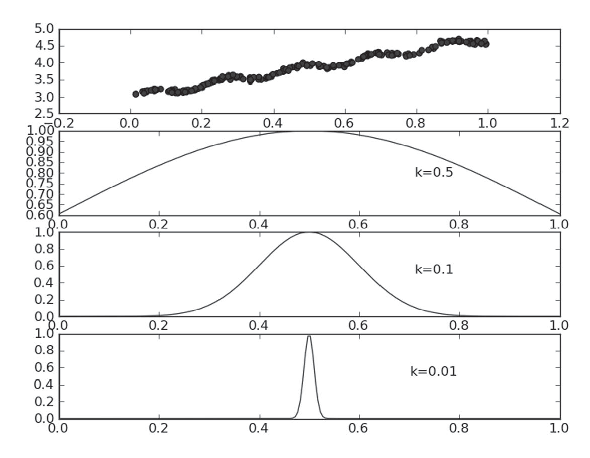
\includegraphics[width=0.55\textwidth]{tau.eps}
  \caption{$~\tau~$的作用范围}
\end{figure}

\noindent实验结果可视化:
\begin{figure}[!h]
  \centering
  \includegraphics[width=0.6\textwidth]{lwlr1.eps}
  \caption{$\tau=1$}
\end{figure}
\begin{figure}[!htb]
  \centering
  \includegraphics[width=0.6\textwidth]{lwlr0_01.eps}
  \caption{$\tau=0.01$}
\end{figure}
\begin{figure}[!htb]
  \centering
  \includegraphics[width=0.6\textwidth]{lwlr0_003.eps}
  \caption{$\tau=0.003$}
\end{figure}\\
分析:\\
从结果来看 局部线性回归能很好地解决线性回归欠拟合的问题,但又可能出现过拟合。\\
所以参数调整影响了模型的泛化能力。选取合适参数至关重要。\\
虽然局部线性回归能增强模型的泛化能力。但是它也有自己的缺陷。就是对每个点的预测都必须使用整个数据集。这样大大增加了计算量。\\

\noindent存在问题:\\
考虑一个问题,当数据特征比训练集样本点还多时,也就是说不可逆,矩阵求导无计可施。此时就要用缩减样本来“理解”数据,求得回归系数矩阵。
即就是:
\begin{equation}\nonumber
\begin{split}
  &R(X^TX)=R(X)=m\\
  &if~\#feature>\#sample ~~(n>m)\\
  &X^TX\in R^{n\times n}\\
  So,&(X^TX)^{-1}~not~exist.
\end{split}
\end{equation}

\subsubsection{示例:利用线性回归预测鲍鱼年龄}
\noindent实战代码以及结果见注释:\\
\noindent程序核心函数代码:
\begin{lstlisting}
def standRegres(xArr,yArr):
    xMat = np.mat(xArr)
    yMat = np.mat(yArr).T
    xTx = xMat.T*xMat  #xMat.T*xMat*w - xMat.T*yMat = 0
    if np.linalg.det(xTx) == 0.0:
        print ("This matrix is singular, cannot do inverse")
        return
    ws = xTx.I * (xMat.T*yMat)
    return ws

def lwlr(testPoint,xArr,yArr,k=1.0):
    xMat = np.mat(xArr); yMat = np.mat(yArr).T
    m = np.shape(xMat)[0]
    weights = np.mat(np.eye((m)))
    for j in range(m):                      #next 2 lines create weights matrix
        diffMat = testPoint - xMat[j,:]   #difference matrix
        weights[j,j] = np.exp(diffMat*diffMat.T/(-2.0*k**2))   #weighted matrix
    xTx = xMat.T * (weights * xMat)
    if np.linalg.det(xTx) == 0.0:
        print ("This matrix is singular, cannot do inverse")
        return
    ws = xTx.I * (xMat.T * (weights * yMat))   #normal equation
    #ws #7 feature,and 1
    return testPoint * ws

#locally weighted linear regression
yHat01 = function.lwlrTest(abX[0:99],abX[0:99],abY[0:99],0.1) #training set #0-99
yHat1 = function.lwlrTest(abX[0:99],abX[0:99],abY[0:99],1)
yHat10 = function.lwlrTest(abX[0:99],abX[0:99],abY[0:99],10)

#error
error01 = function.rssError(abY[0:99],yHat01.T)   #56.820227823572182
error1 = function.rssError(abY[0:99],yHat1.T)   #429.89056187016683
error10 = function.rssError(abY[0:99],yHat10.T)   #549.1181708825128

#generalization
yHat01g = function.lwlrTest(abX[100:199],abX[100:199],abY[100:199],0.1) #test set #100-199
yHat1g = function.lwlrTest(abX[100:199],abX[100:199],abY[100:199],1)
yHat10g = function.lwlrTest(abX[100:199],abX[100:199],abY[100:199],10)

#error
error01g = function.rssError(abY[100:199],yHat01g.T)   #36199.797699875046
error1g = function.rssError(abY[100:199],yHat1g.T)   #231.81344796874004
error10g = function.rssError(abY[100:199],yHat10g.T)   #291.87996390562728

#compare
#k = 0.1 overfitting

#linear regression
ws = function.standRegres(abX[0:99],abY[0:99])
yHat = np.mat(abX[100:199])*ws
errorlr = function.rssError(yHat.T.A,abY[100:199])   #518.63631532510897

#compare
#lwlr is better than lr
\end{lstlisting}

%\subsection{缩减系数来理解数据}